\documentclass[
	% -- opções da classe memoir --
	12pt,				% tamanho da fonte
	openright,			% capítulos começam em pág ímpar (insere página vazia caso preciso)
	twoside,			% para impressão em recto e verso. Oposto a oneside
	a4paper,			% tamanho do papel. 
	% -- opções da classe abntex2 --
	%chapter=TITLE,		% títulos de capítulos convertidos em letras maiúsculas
	%section=TITLE,		% títulos de seções convertidos em letras maiúsculas
	%subsection=TITLE,	% títulos de subseções convertidos em letras maiúsculas
	%subsubsection=TITLE,% títulos de subsubseções convertidos em letras maiúsculas
	% -- opções do pacote babel --
	english,			% idioma adicional para hifenização
	french,				% idioma adicional para hifenização
	spanish,			% idioma adicional para hifenização
	brazil,				% o último idioma é o principal do documento
]{abntex2}

% ---
% PACOTES
% ---

% ---
% Pacotes fundamentais 
% ---
\usepackage{lmodern}			% Usa a fonte Latin Modern
\usepackage[T1]{fontenc}		% Selecao de codigos de fonte.
\usepackage[utf8]{inputenc}		% Codificação do documento (conversão automática dos acentos)
\usepackage{indentfirst}		% Indenta o primeiro parágrafo de cada seção.
\usepackage{color}				% Controle das cores
\usepackage{graphicx}			% Inclusão de gráficos
%\usepackage[draft]{graphicx}
\usepackage{microtype} 			% para melhorias de justificação
% ---

% ---
% Pacotes de citações
% ---
\usepackage[brazilian,hyperpageref]{backref}	 % Paginas com as citações na bibl
\usepackage[alf]{abntex2cite}	% Citações padrão ABNT

\usepackage{subfig}
\graphicspath{{img/}}

\usepackage{amsmath, amsfonts, amssymb}
\DeclareMathOperator{\sen}{sen}
\DeclareMathOperator{\tg}{tg}
\DeclareMathOperator{\cossec}{cossec}
\DeclareMathOperator{\cotg}{cotg}
\DeclareMathOperator{\arcsen}{arcsen}
\DeclareMathOperator{\arctg}{arctg}
\DeclareMathOperator{\arcsec}{arcsec}
\DeclareMathOperator{\arccossec}{arccossec}
\DeclareMathOperator{\arccotg}{arccotg}
\DeclareMathOperator{\e}{e}

\usepackage[normalem]{ulem}
\newcommand{\overstrike}[1]{\ifmmode\text{\sout{\ensuremath{#1}}}\else\sout{#1}\fi}

% --- 
% CONFIGURAÇÕES DE PACOTES
% --- 

% ---
% Configurações do pacote backref
% Usado sem a opção hyperpageref de backref
\renewcommand{\backrefpagesname}{Citado na(s) página(s):~}
% Texto padrão antes do número das páginas
\renewcommand{\backref}{}
% Define os textos da citação
\renewcommand*{\backrefalt}[4]{
	\ifcase #1 %
	Nenhuma citação no texto.%
	\or
	Citado na página #2.%
	\else
	Citado #1 vezes nas páginas #2.%
	\fi}%
% ---

% ---
% Informações de dados para CAPA e FOLHA DE ROSTO
% ---
\title{Curso de integrais duplas e triplas}
\author{César Antônio de Magalhães}
\local{Brasil}
\data{2016}
\instituicao{%
	Universidade Norte do Paraná -- Unopar}
\tipotrabalho{Exercício}
% O preambulo deve conter o tipo do trabalho, o objetivo, 
% o nome da instituição e a área de concentração 
\preambulo{Exercícios de integrais duplas e triplas em conformidade
	com as normas ABNT.}

% ---
% Configurações de aparência do PDF final

% alterando o aspecto da cor azul
\definecolor{blue}{RGB}{41,5,195}

% informações do PDF
\makeatletter
\hypersetup{
	%pagebackref=true,
	pdftitle={\@title}, 
	pdfauthor={\@author},
	pdfsubject={\imprimirpreambulo},
	pdfcreator={LaTeX with abnTeX2},
	pdfkeywords={abnt}{latex}{abntex}{abntex2}{projeto de pesquisa}, 
	colorlinks=true,       		% false: boxed links; true: colored links
	linkcolor=blue,          	% color of internal links
	citecolor=blue,        		% color of links to bibliography
	filecolor=magenta,      		% color of file links
	urlcolor=blue,
	bookmarksdepth=4
}
\makeatother
% ---

% --- 
% Espaçamentos entre linhas e parágrafos 
% --- 

% O tamanho do parágrafo é dado por:
\setlength{\parindent}{1.3cm}

% Controle do espaçamento entre um parágrafo e outro:
\setlength{\parskip}{0.2cm}  % tente também \onelineskip

% ---
% compila o indice
% ---
\makeindex
% ---

% ----
% Início do documento
% ----
\begin{document}

% Seleciona o idioma do documento (conforme pacotes do babel)
%\selectlanguage{english}
\selectlanguage{brazil}

% Retira espaço extra obsoleto entre as frases.
\frenchspacing 

% ----------------------------------------------------------
% ELEMENTOS PRÉ-TEXTUAIS
% ----------------------------------------------------------
% \pretextual

% ---
% Capa
% ---
\imprimircapa
% ---

% ---
% Folha de rosto
% ---
\imprimirfolhaderosto
% ---

% ---
% NOTA DA ABNT NBR 15287:2011, p. 4:
%  ``Se exigido pela entidade, apresentar os dados curriculares do autor em
%     folha ou página distinta após a folha de rosto.''
% ---

% ---
% inserir lista de ilustrações
% ---
\pdfbookmark[0]{\listfigurename}{lof}
\listoffigures*
\cleardoublepage
% ---

% ---
% inserir lista de tabelas
% ---
\pdfbookmark[0]{\listtablename}{lot}
\listoftables*
\cleardoublepage
% ---

% ---
% inserir lista de abreviaturas e siglas
% ---
\begin{siglas}
	\item[ABNT] Associação Brasileira de Normas Técnicas
	\item[$ f(x),\, g(x),\, f(y),\, g(y),\, f(x,y),\, \textrm{...} $] Função
	\item[$ dx,\, dy,\, d\theta,\, \textrm{...} $] Derivada
	\item[$ v $] Volume
	\item[$ a $] Área
	\item[$ R $] Região
	\item[$ P $] Ponto
	\item[$ r $] Raio
	\item[$ co $] Cateto oposto
	\item[$ ca $] Cateto adjacente
	\item[$ h $] Hipotenusa
	\item[$\sen$] Seno
	\item[$ \cos $] Cosseno
	\item[$ \tg $] Tangente
	\item[$ \sec $] Secante
	\item[$ \cossec $] Cossecante
	\item[$ \cotg $] Cotangente
	\item[$ \arcsen $] Arco seno
	\item[$ \arccos $] Arco cosseno
	\item[$ \arctg $] Arco tangente
	\item[$ \arcsec $] Arco secante
	\item[$ \arccossec $] Arco cossecante
	\item[$ \arccotg $] Arco cotangente
	\item[$ \log $] Logaritmo
	\item[$ \ln $] Logaritmo natural
	\item[$ \e $] Número de Euler
	\item[$ \lim $] Limite	
\end{siglas}
% ---

% ---
% inserir lista de símbolos
% ---
\begin{simbolos}
	\item[$ \displaystyle\int $] Integral
	\item[$ \displaystyle\iint $] Integral dupla
	\item[$ \pi $] Letra grega minúscula pi
	\item[$ \alpha $] Ângulo alfa
	\item[$ \theta $] Ângulo theta
	\item[$ \in $] Pertence
\end{simbolos}
% ---

% ---
% inserir o sumário
% ---
\pdfbookmark[0]{\contentsname}{toc}
\tableofcontents*
\cleardoublepage
% ---


% ----------------------------------------------------------
% ELEMENTOS TEXTUAIS
% ----------------------------------------------------------
\textual

% ----------------------------------------------------------
% Introdução
% ----------------------------------------------------------
\chapter*[Introdução]{Introdução}
\addcontentsline{toc}{chapter}{Introdução}

Esse documento contém exercícios retirados do Youtube através do canal OMatematico.com, acesse-o em \url{https://www.youtube.com/c/omatematicogrings}. 

Uma lista de exercícios prontos sobre \emph{derivadas duplas e triplas} é apresentado em \citeonline{curso_integrais_duplas_triplas}.

% ----------------------------------------------------------
% Capitulo de textual  
% ----------------------------------------------------------

\chapter{Integrais duplas}\label{integrais_duplas}
\chapterprecis{Cálculo de integrais duplas.}\index{sinopse de capítulo}

\section{Invertendo os limites de integração - Aula 1}			
	\begin{enumerate}
	\item Exercício
	
	\begin{figure}[H]
		\caption{Integrais duplas - Aula 1 - Exercício I e II}
		\label{v01_a01_e01}
		\centering
		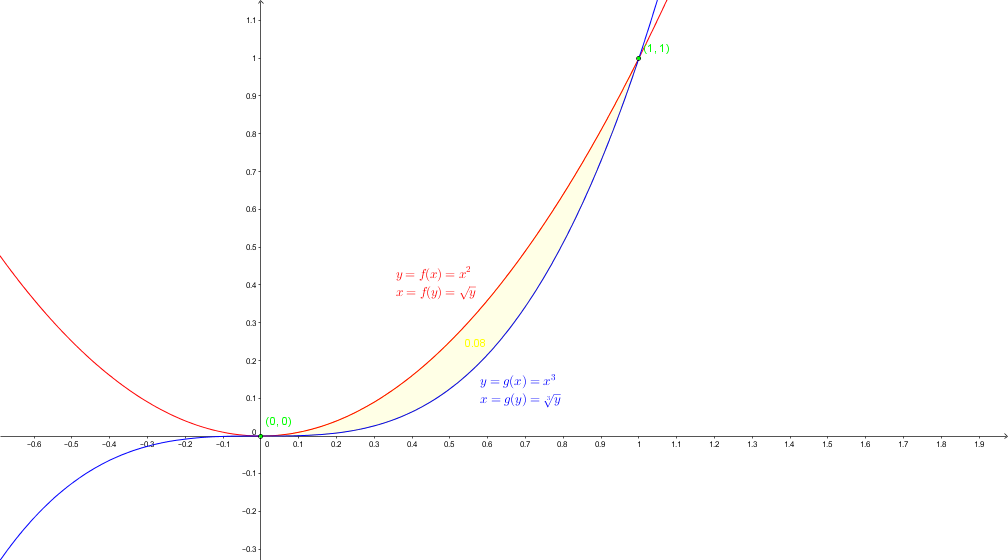
\includegraphics[width=\textwidth]{v01_a01_e01.png}		
	\end{figure}
				
	$f(x) = x^2;\; g(x) = x^3$\newline
	$x = 0 \Rightarrow f(0) = g(0) \Rightarrow 0^2 = 0^3$\newline
	$x = 1 \Rightarrow f(1) = g(1) \Rightarrow 1^2 = 1^3$\newline
	
	$a = \integral_0^1 dx \integral_{g(x)}^{f(x)} dy = \integral_0^1 dx \integral_{x^3}^{x^2} dy = \integral_0^1 dx\, [y]_{x^3}^{x^2} = \integral_0^1 dx \left[x^2 - x^3\right] = \integral_0^1 x^2\, dx - \integral_0^1 x^3\, dx = \left[\dfrac{x^3}{3} - \dfrac{x^4}{4}\right]_0^1 = \left[\dfrac{4x^3 - 3x^2}{12}\right]_0^1 = \dfrac{1}{12}\left[4x^3 - 3x^2\right]_0^1 = \dfrac{1}{12}\left[x^2\left(4x - 3\right)\right]_0^1 = \dfrac{1}{12}\left[1^2\left(4 \cdot 1 - 3\right) \overstrike{- 0^2\left(4 \cdot 0 - 3\right)}\right] = \dfrac{1}{12} = 0,08\overline{3}$
					
	\item Exercício
	
	$f(x) = x^2 \Rightarrow f(y) = \sqrt{y};\; g(x) = x^3 \Rightarrow g(y) = \sqrt[3]{y}$\newline
	$y = 0 \Rightarrow f(0) = g(0) \Rightarrow \sqrt{0} = \sqrt[3]{0}$\newline
	$y = 1 \Rightarrow f(1) = g(1) \Rightarrow \sqrt{1} = \sqrt[3]{1}$\newline
	
	$a = \integral_0^1 dy \integral_{f(y)}^{g(y)} dx = \integral_0^1 dy \integral_{\sqrt{y}}^{\sqrt[3]{y}} dx = \integral_0^1 dy\, [x]_{\sqrt{y}}^{\sqrt[3]{y}} = 
	\integral_0^1 dy \left[\sqrt[3]{y} - \sqrt{y}\right] = \integral_0^1 \sqrt[3]{y}\, dy - \integral_0^1 \sqrt{y}\, dy = \integral_0^1 y^{\frac{1}{3}}\, dy - \integral_0^1 y^{\frac{1}{2}}\, dy = \left[\dfrac{y^{\frac{4}{3}}}{\left(\dfrac{4}{3}\right)} - \dfrac{y^{\frac{3}{2}}}{\left(\dfrac{3}{2}\right)}\right]_0^1 = \left[\dfrac{3 \sqrt[3]{y^4}}{4} - \dfrac{2 \sqrt{y^3}}{3}\right]_0^1 = \left[\dfrac{9 \sqrt[3]{y^4} - 8 \sqrt{y^3}}{12}\right]_0^1 = \dfrac{1}{12}\left[9 \sqrt[3]{y^4} - 8 \sqrt{y^3}\right]_0^1 =\\ \dfrac{1}{12}\left[\left(9 \sqrt[3]{1^4} - 8 \sqrt{1^3}\right) \overstrike{-\left(9 \sqrt[3]{0^4} - 8 \sqrt{0^3}\right)}\right] = \dfrac{1}{12}(9 - 8) = \dfrac{1}{12} = 0,08\overline{3}$
\end{enumerate}		
\section{Determinação da região de integração - Aula 2}		
	\begin{enumerate}
	\item Exercício
	
	$R = \left\{(x, y) \in \mathbb{R}^2 \,|\, 0 \leq x \leq 2 \,,\, 0 \leq y \leq 6 \right\}$
	
	\begin{figure}[H]
		\caption{Integrais duplas - Aula 2 - Exercício I}
		\label{v02_a02_e01}
		\centering
		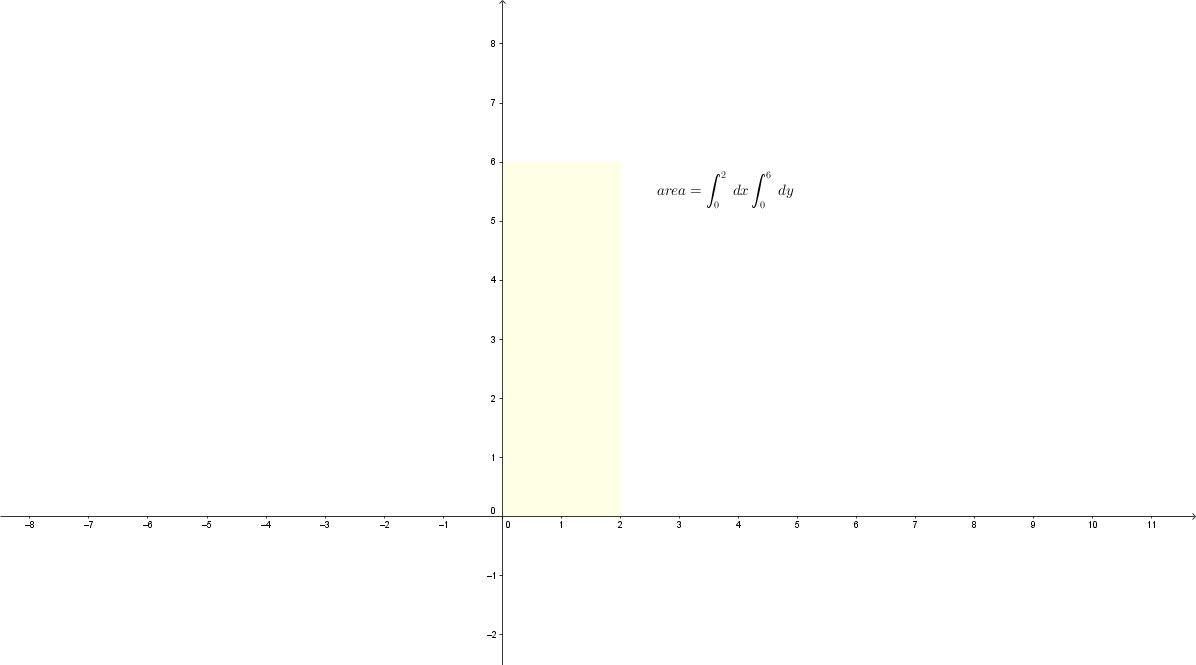
\includegraphics[width=\textwidth]{v02_a02_e01.png}		
	\end{figure}
	
	$a = \integral_0^2 dx \integral_0^6 dy = \integral_0^2 dx\, [y]_0^6 = \integral_0^2 dx\, [6 - 0] = 6\integral_0^2 dx = 6[x]_0^2 = 6[2 - 0] = 6 \cdot 2 = 12$
	
	\item Exercício
	
	$R = \left\{(x, y) \in \mathbb{R}^2 \,|\, 0 \leq x \leq 1 \,,\, x \leq y \leq 2x \right\}$
						
	\begin{figure}[H]
		\caption{Integrais duplas - Aula 2 - Exercício II}
		\label{v02_a02_e02}
		\centering
		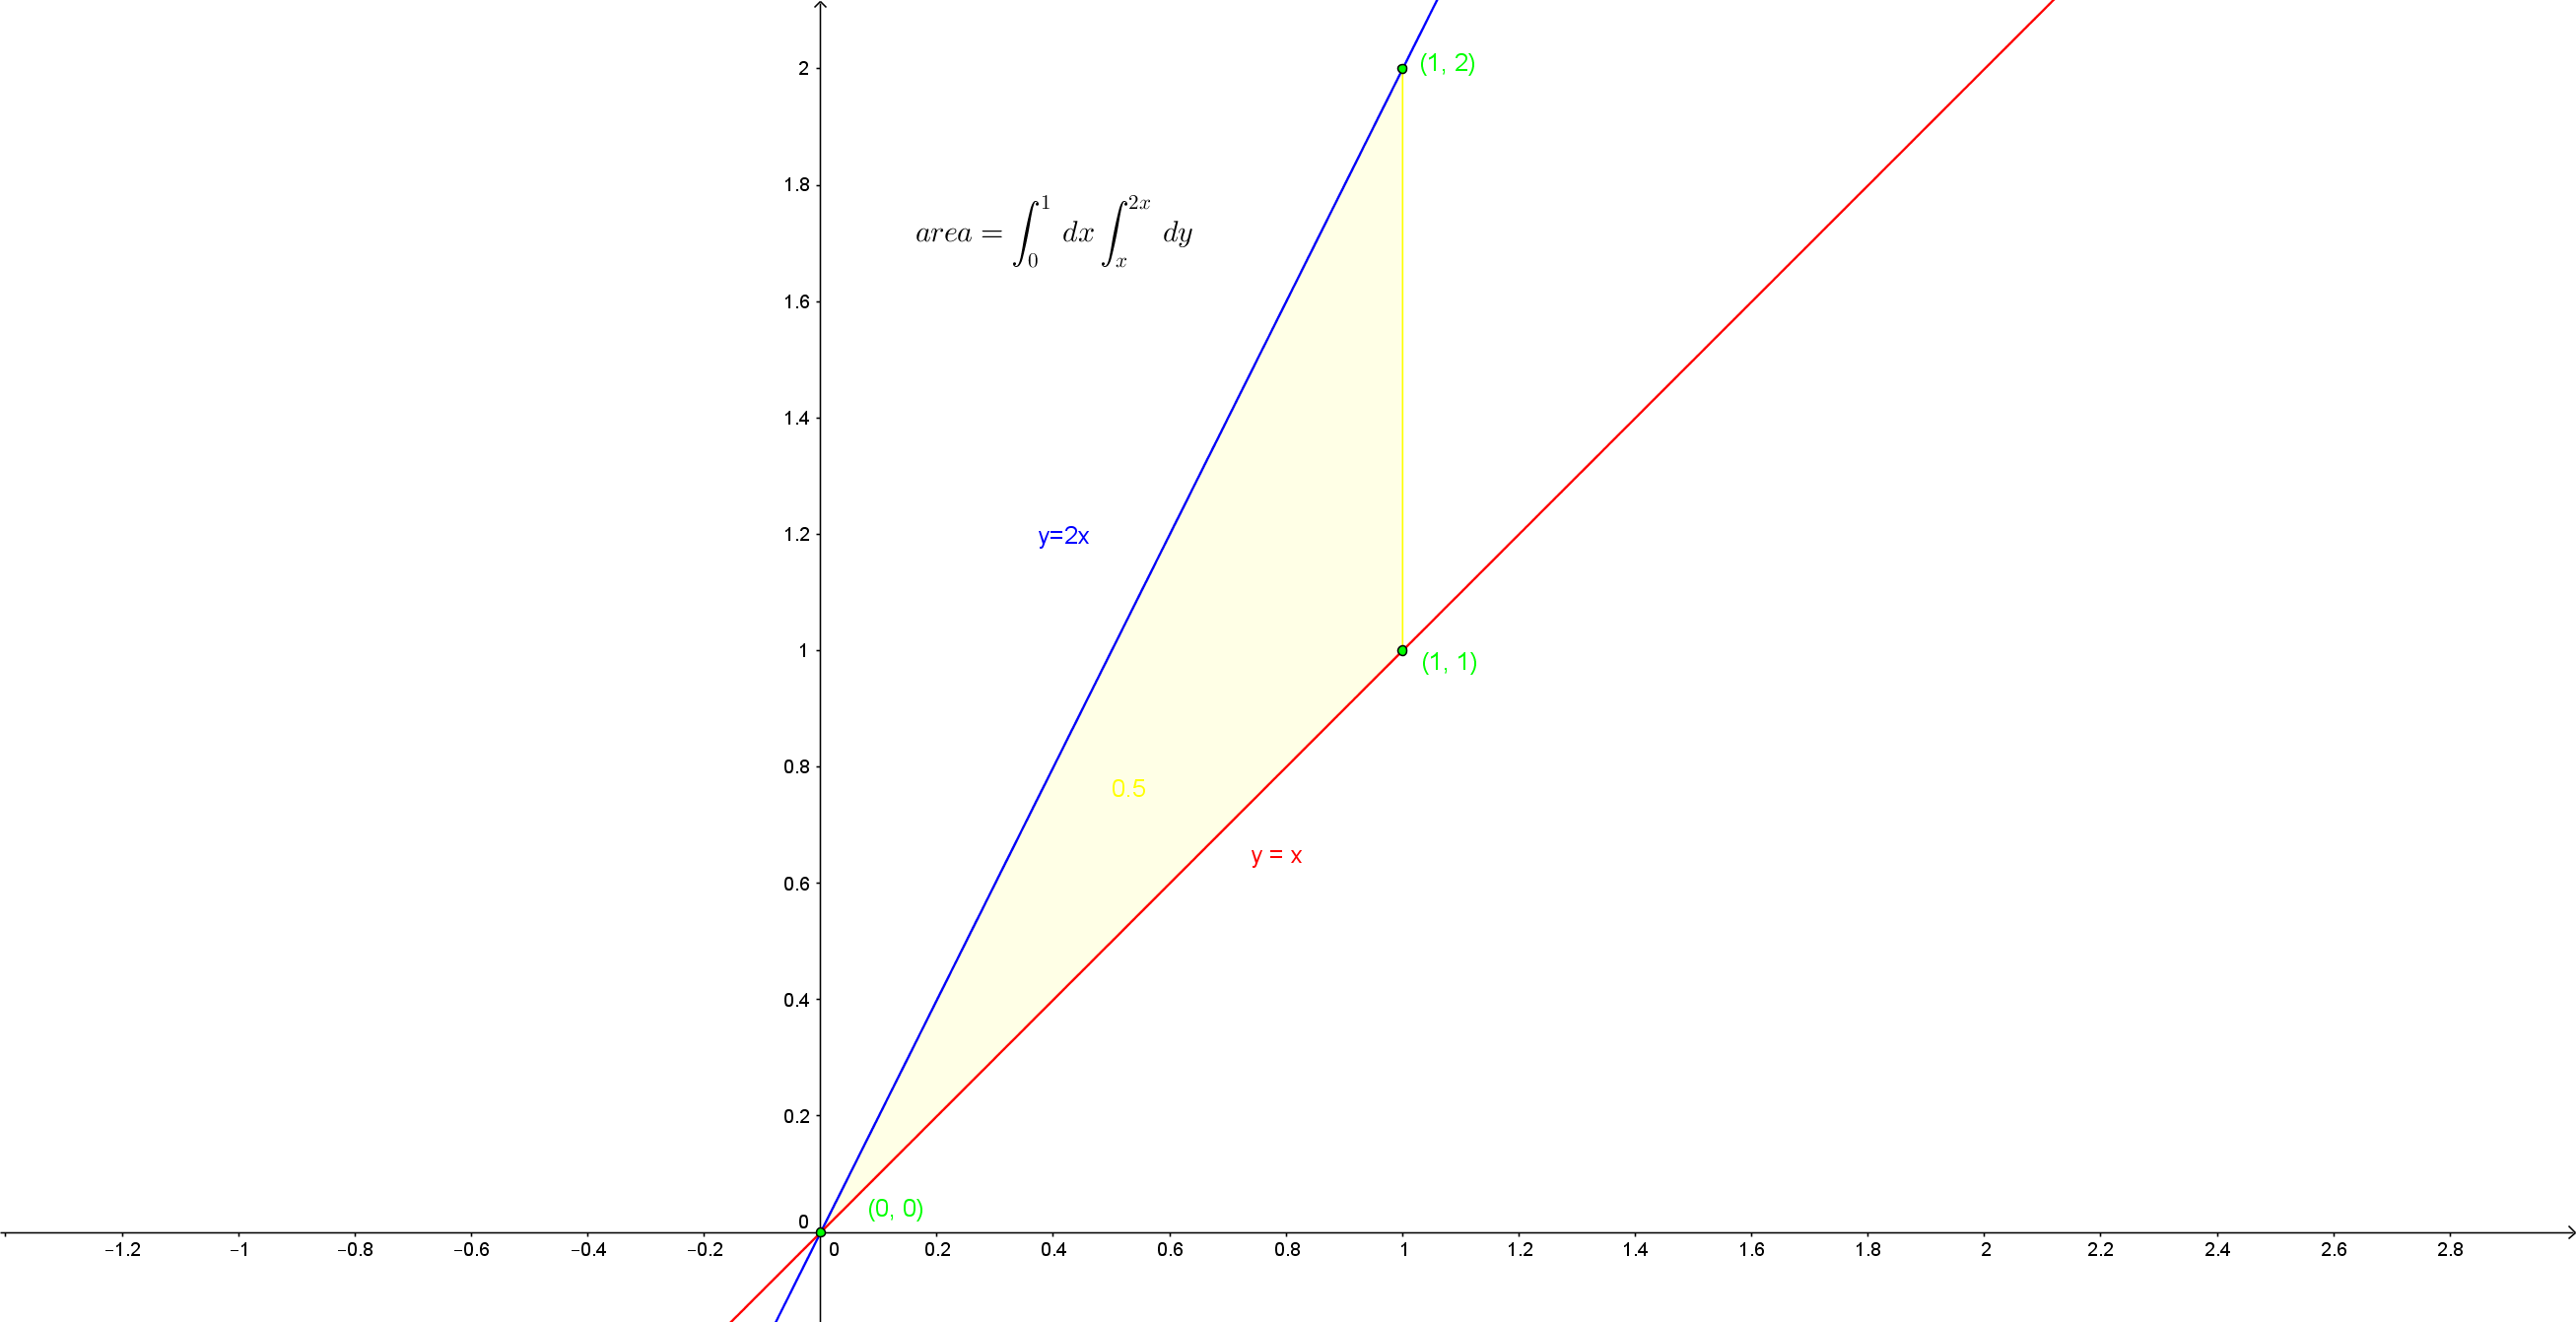
\includegraphics[width=\textwidth]{v02_a02_e02.png}		
	\end{figure}
	
	$a = \integral_0^1 dx \integral_{x}^{2x} dy = \integral_0^1 dx\, [y]_{x}^{2x} = \integral_0^1 dx\, [2x - x] = 2\integral_0^1 x\, dx - \integral_0^1 x\, dx = \left[\overstrike{2}\dfrac{x^2}{\overstrike{2}} - \dfrac{x^2}{2}\right]_0^1 = \left[\dfrac{2x^2 - x^2}{2}\right]_0^1 = \dfrac{1}{2}\left[x^2\right]_0^1 = \dfrac{1}{2}\left[1^2 \overstrike{- 0^2}\right] = \dfrac{1}{2} = 0,5 $
	
	\item Exercício
	
	$R = \left\{(x, y) \in \mathbb{R}^2 \,|\, 0 \leq y \leq 1 \,,\, 0 \leq x \leq \sqrt{1 - y^2} \right\}$
	
	$y = 0,\, y=1$\newline
	$x = 0,\, x = \sqrt{1 - y^2} \Rightarrow x^2 = 1 - y^2 \Rightarrow x^2 - 1 = -y^2 \Rightarrow y^2 = -x^2 + 1 \Rightarrow y = \sqrt{1 -x^2}$
					
	\begin{figure}[H]
		\caption{Integrais duplas - Aula 2 - Exercício III}
		\label{v02_a02_e03}
		\centering
		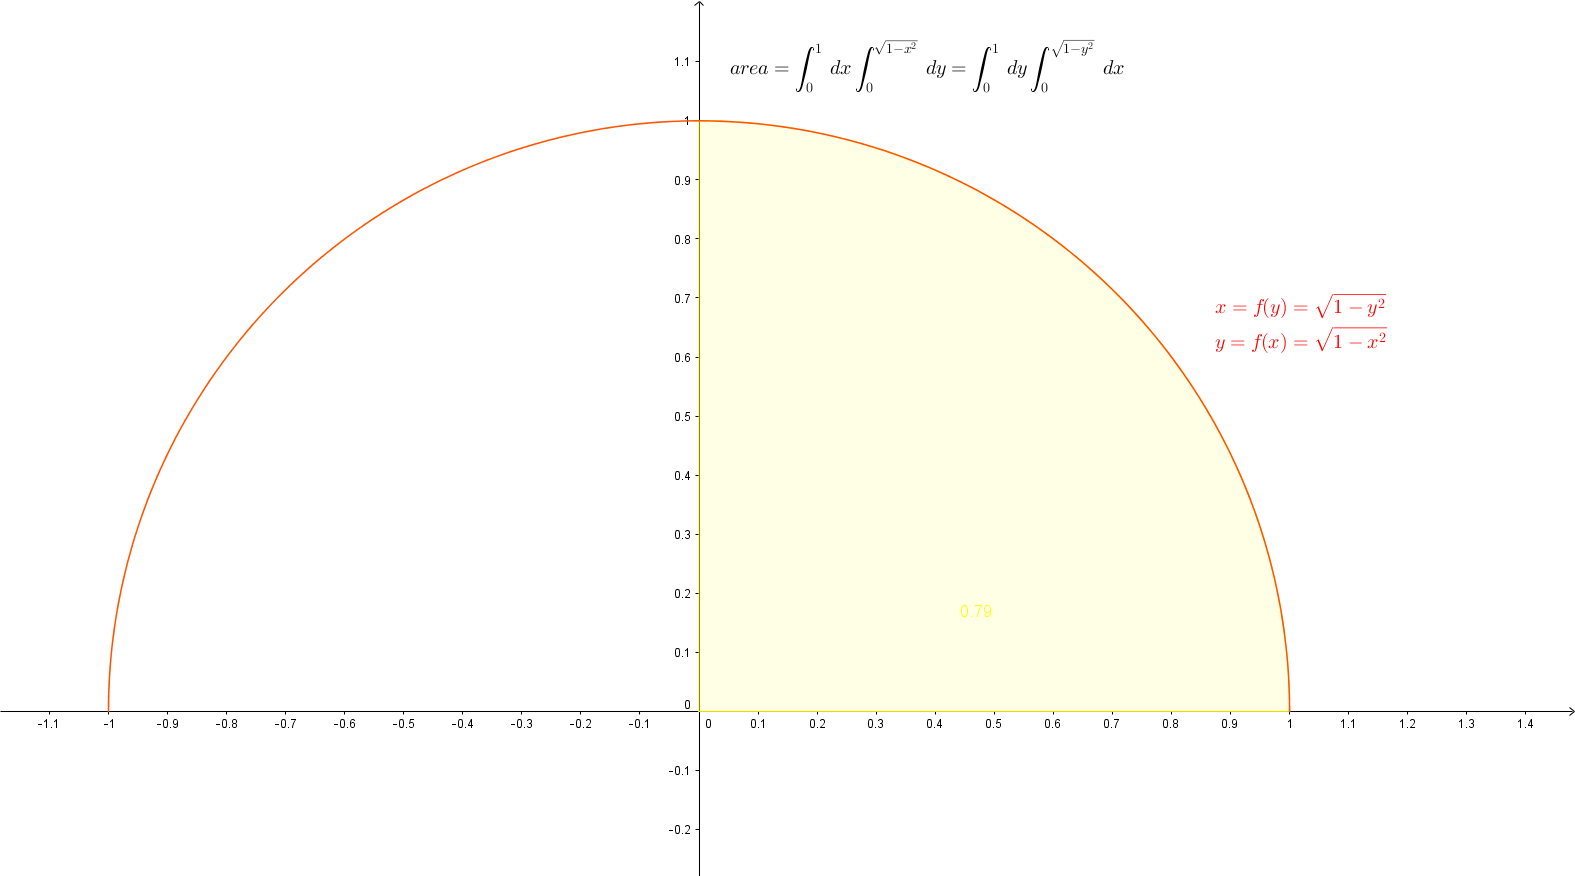
\includegraphics[width=\textwidth]{v02_a02_e03.png}		
	\end{figure}
	
	$a = \integral_0^1 dy \integral_0^{f(y)} dx = \integral_0^1 dy \integral_0^{\sqrt{1 - y^2}} dx = \integral_0^1 dy\, [x]_0^{\sqrt{1 - y^2}} = \integral_0^1 dy\, \left[\sqrt{1 - y^2} - 0\right] = \integral_0^1 \sqrt{1 - y^2}\, dy = \integral_0^1 \sqrt{1 - \sen^2(t)}\, \cos(t) dt = \integral_0^1 \sqrt{\cos^2(t)}\, \cos(t) dt = \integral_0^1 \cos(t)\cos(t) dt = \integral_0^1 \cos^2(t) dt = \integral_0^1 \dfrac{1 + \cos(2t)}{2} dt = \dfrac{1}{2}\integral_0^1 \left[1 + \cos(2t)\right] dt = \dfrac{1}{2}\integral_0^1 dt + \dfrac{1}{2}\integral_0^1 \cos(2t) dt = \dfrac{1}{2}\integral_0^1 dt + \dfrac{1}{2}\integral_0^1 \cos(u) \dfrac{du}{2} = \dfrac{1}{2}\integral_0^1 dt + \dfrac{1}{4}\integral_0^1 \cos(u)\, du = \left[\dfrac{1}{2}t + \dfrac{1}{4}\sen(u)\right]_0^1 = \left[\dfrac{t}{2} + \dfrac{\sen(2t)}{4}\right]_0^1 = \left[\dfrac{t}{2} + \dfrac{2\sen(t)\cos(t)}{4}\right]_0^1 = \left[\dfrac{t + \sen(t)\cos(t)}{2}\right]_0^1 = \dfrac{1}{2}\left[\arcsen(y) + y\sqrt{1 - y^2}\right]_0^1 =\\ \dfrac{1}{2}\left[\left(\arcsen(1) \overstrike{+ 1 \cdot\sqrt{1 - 1^2}}\right) - \left(\arcsen(0) \overstrike{+ 0 \cdot \sqrt{1 - 0^2}}\right)\right] = \dfrac{1}{2}\left[\dfrac{\pi}{2} - 0\right] = \dfrac{\pi}{4} = 0,785$ \newline\newline
	$y = \sen(t) \Rightarrow dy = \cos(t) dt$\newline
	$u = 2t \Rightarrow \dfrac{du}{2} = dt$\newline\newline
	$\sen(t) = \dfrac{co}{h} = \dfrac{y}{1} = y$\newline
	$h^2 = co^2 + ca^2 \Rightarrow 1 = y^2 + ca^2 \Rightarrow ca = \sqrt{1 - y^2}$\newline
	$\cos(t) = \dfrac{ca}{h} = \dfrac{\sqrt{1 - y^2}}{1} = \sqrt{1 - y^2}$\newline
	$y = \sen(t) \Rightarrow t = \arcsen(y)$
	
	\item Exercício
	
	$y = x^2 + 1 ,\, y = -x^2 - 1 ;\; x = 1 ,\, x = -1$\newline
	$R = \left\{(x, y) \in \mathbb{R}^2 \,|\, -1 \leq x \leq 1 \,,\, -x^2 - 1 \leq y \leq x^2 + 1 \right\}$
	
	\begin{figure}[H]
		\caption{Integrais duplas - Aula 2 - Exercício IV}
		\label{v02_a02_e04}
		\centering
		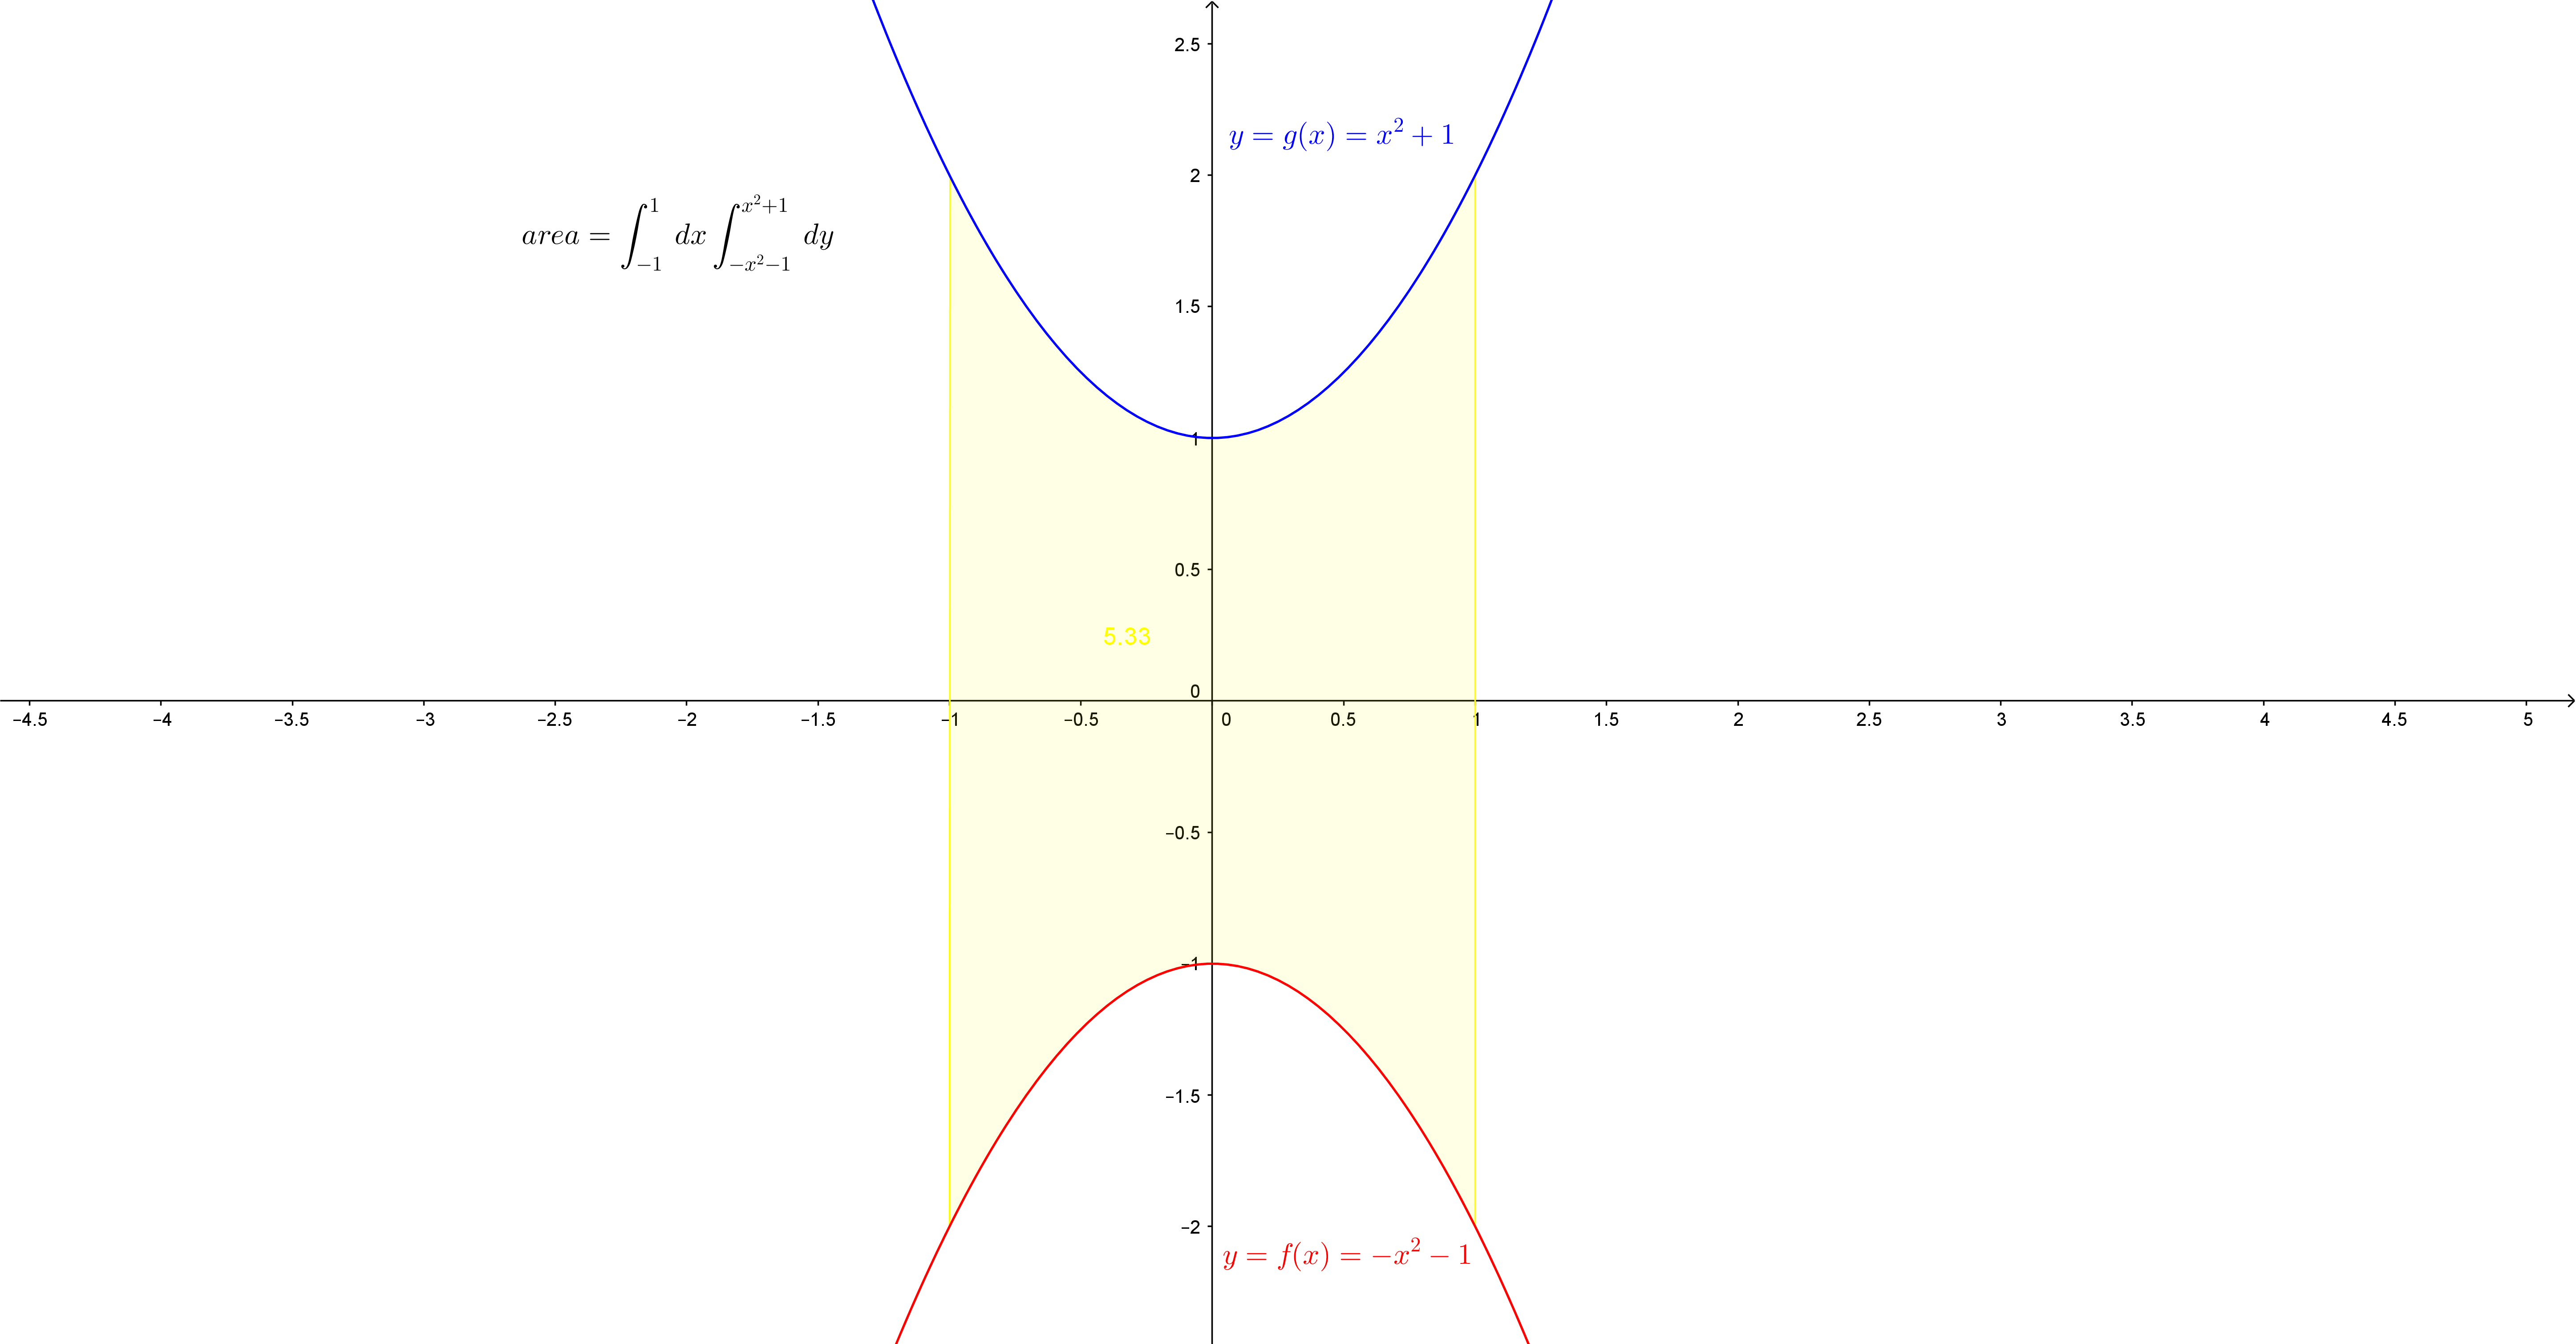
\includegraphics[width=\textwidth]{v02_a02_e04.png}		
	\end{figure}
	
	$a = \integral_{-1}^1 dx \integral_{f(x)}^{g(x)} dy = \integral_{-1}^1 dx \integral_{-x^2 - 1}^{x^2 + 1} dy = \integral_{-1}^1 dx\, [y]_{-x^2 - 1}^{x^2 + 1} = \integral_{-1}^1 dx\, \left[x^2 + 1 - \left(-x^2 - 1\right)\right] = \integral_{-1}^1 dx\, \left[x^2 + 1 + x^2 + 1\right] = \integral_{-1}^1 dx\, \left[2x^2 + 2\right] = 2\integral_{-1}^1 x^2\, dx + 2\integral_{-1}^1 dx = \left[2\dfrac{x^3}{3} +  2x\right]_{-1}^1 = \left[2\left(\dfrac{x^3 + 3x}{3}\right)\right]_{-1}^1 = \dfrac{2}{3}\left[x\left(x^2 + 3\right)\right]_{-1}^1 = \\ \dfrac{2}{3}\left[1 \cdot \left(1^2 + 3\right) - (-1)\left((-1)^2 + 3\right)\right] = \dfrac{2}{3}(4 + 4) = \dfrac{2}{3}8 = \dfrac{16}{3} = 5,\overline{3}$
	
	\item Exercício
	
	$R = \left\{(x, y) \in \mathbb{R}^2 \,|\, 0 \leq y \leq 2 \,,\, -y \leq x \leq y \right\}$
	
	\begin{figure}[H]
		\caption{Integrais duplas - Aula 2 - Exercício V}
		\label{v02_a02_e05}
		\centering
		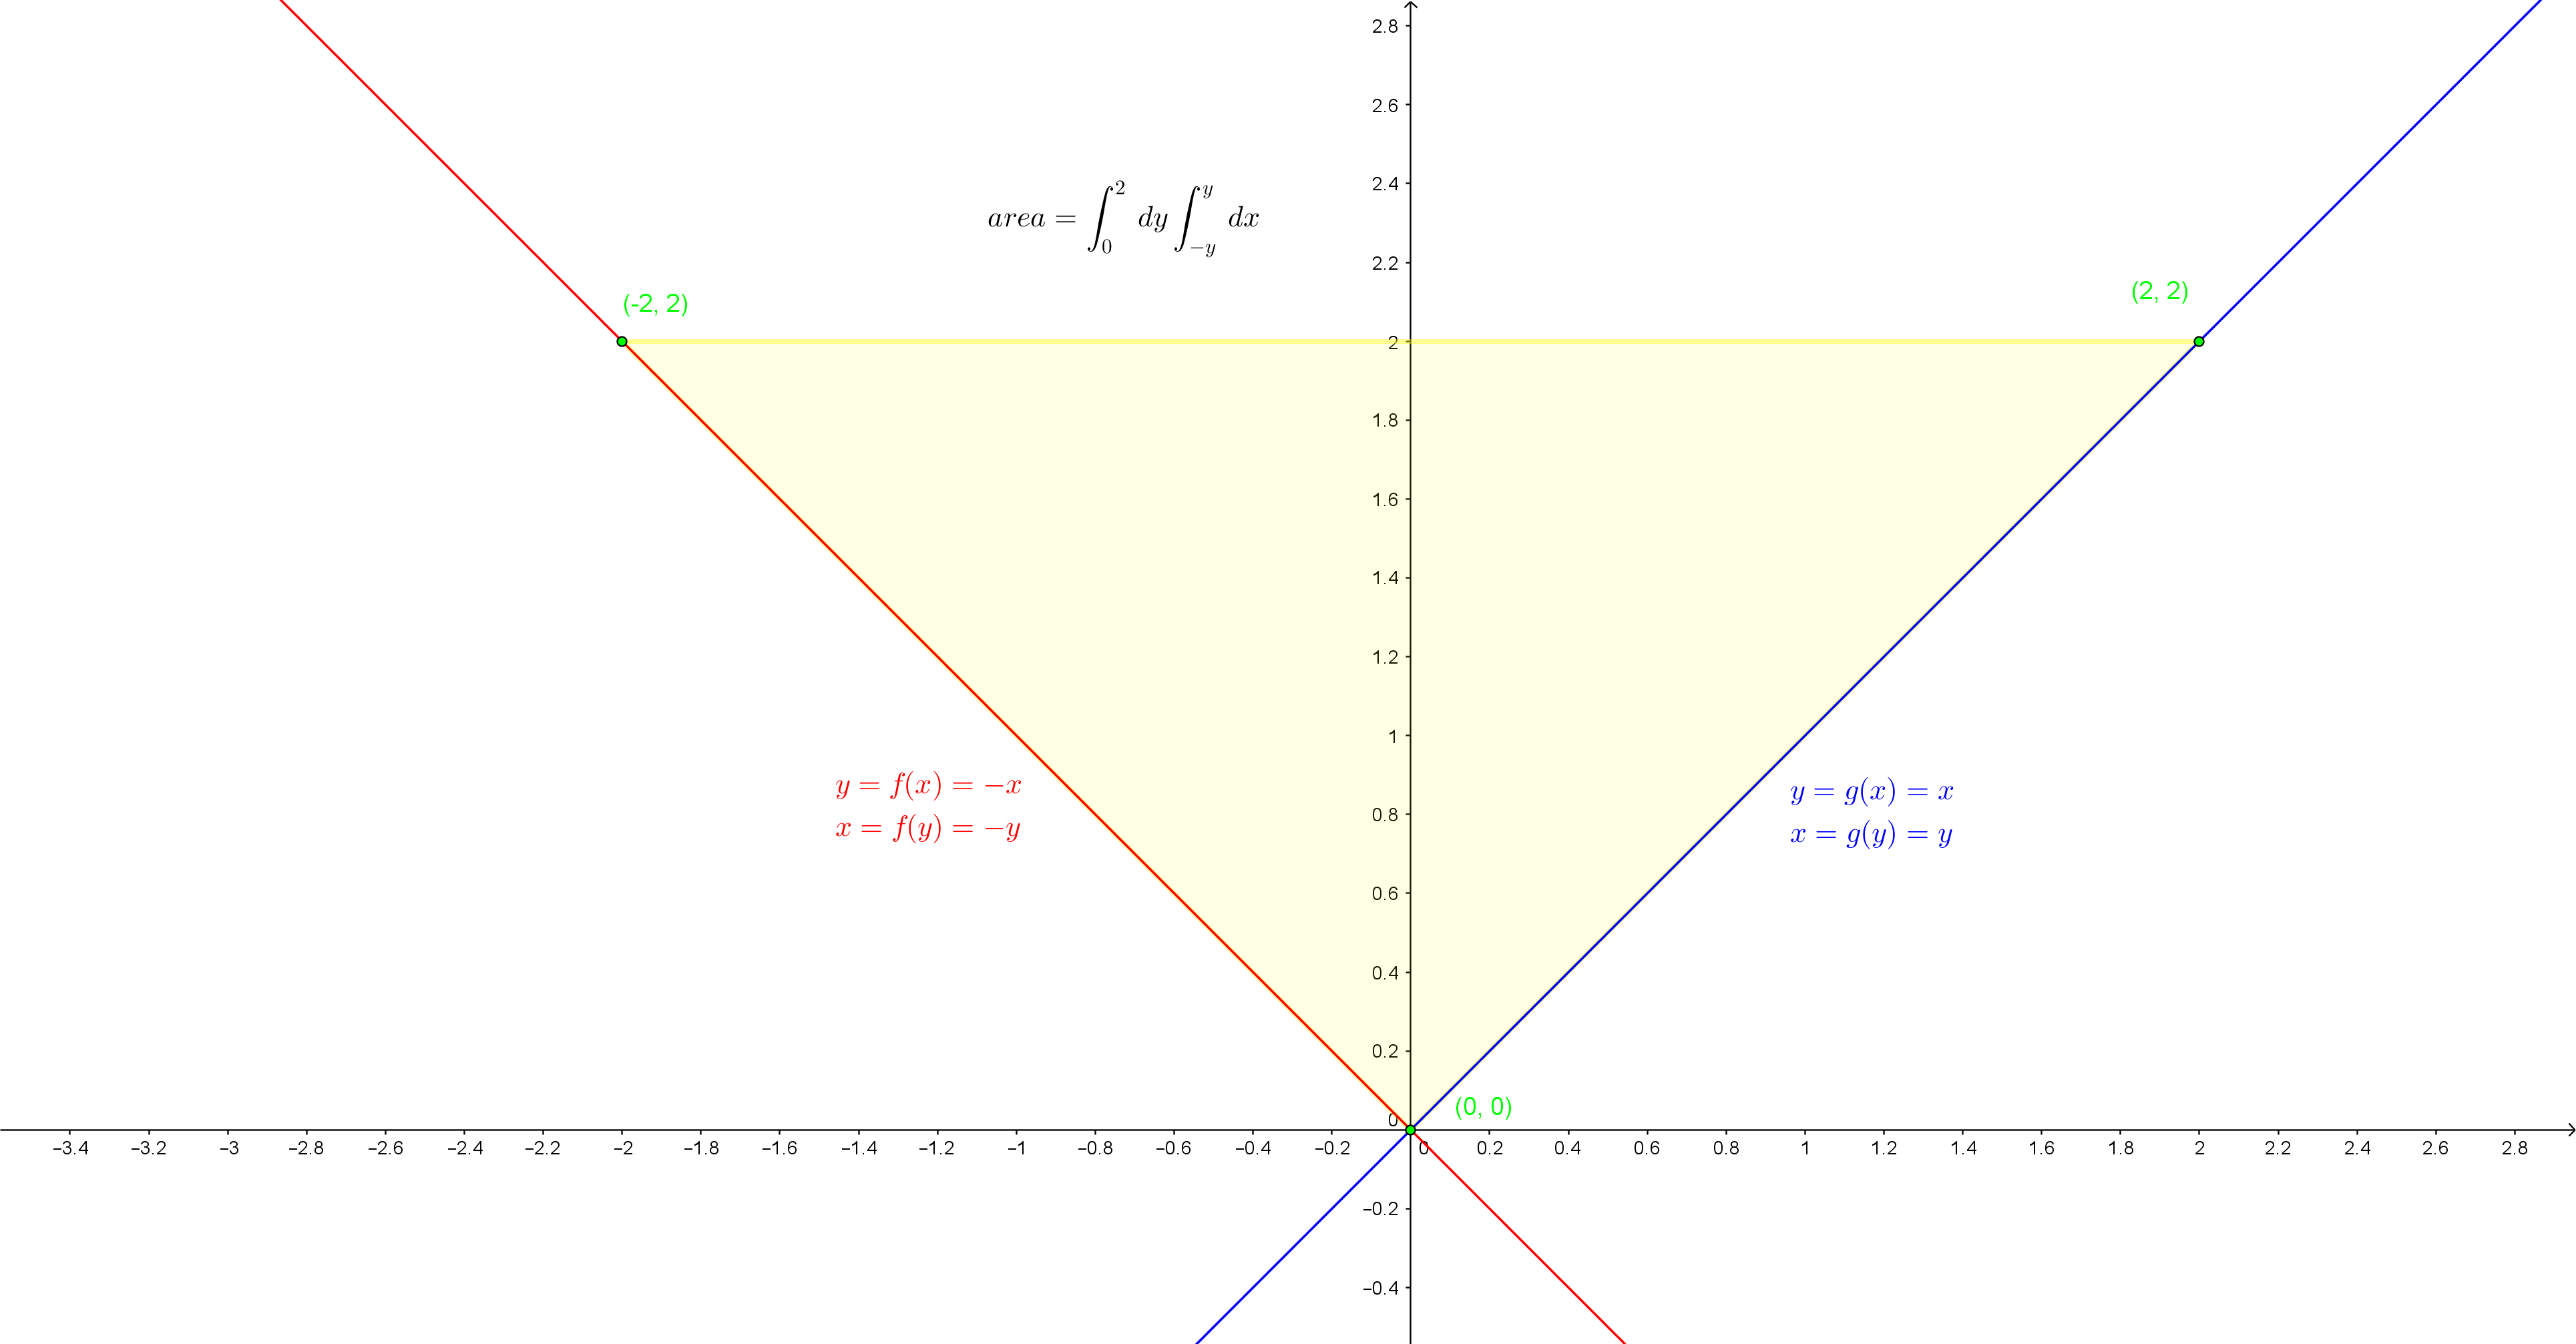
\includegraphics[width=\textwidth]{v02_a02_e05.png}		
	\end{figure}
	
	$a = \integral_0^2 dy \integral_{f(y)}^{g(y)} dx = \integral_0^2 dy \integral_{-y}^y dx = \integral_0^2 dy\, [x]_{-y}^y = \integral_0^2 dy\, [y - (-y)] = \integral_0^2 dy\, [2y] = 2\integral_0^2 y\, dy = \left[\overstrike{2}\frac{y^2}{\overstrike{2}}\right]_0^2 = 2^2 - 0^2 = 4$	
\end{enumerate}		
\section{Cálculo de volume - Aula 3}
	\begin{enumerate}
	\item Exercício
	
	\begin{figure}[H]
		\centering
		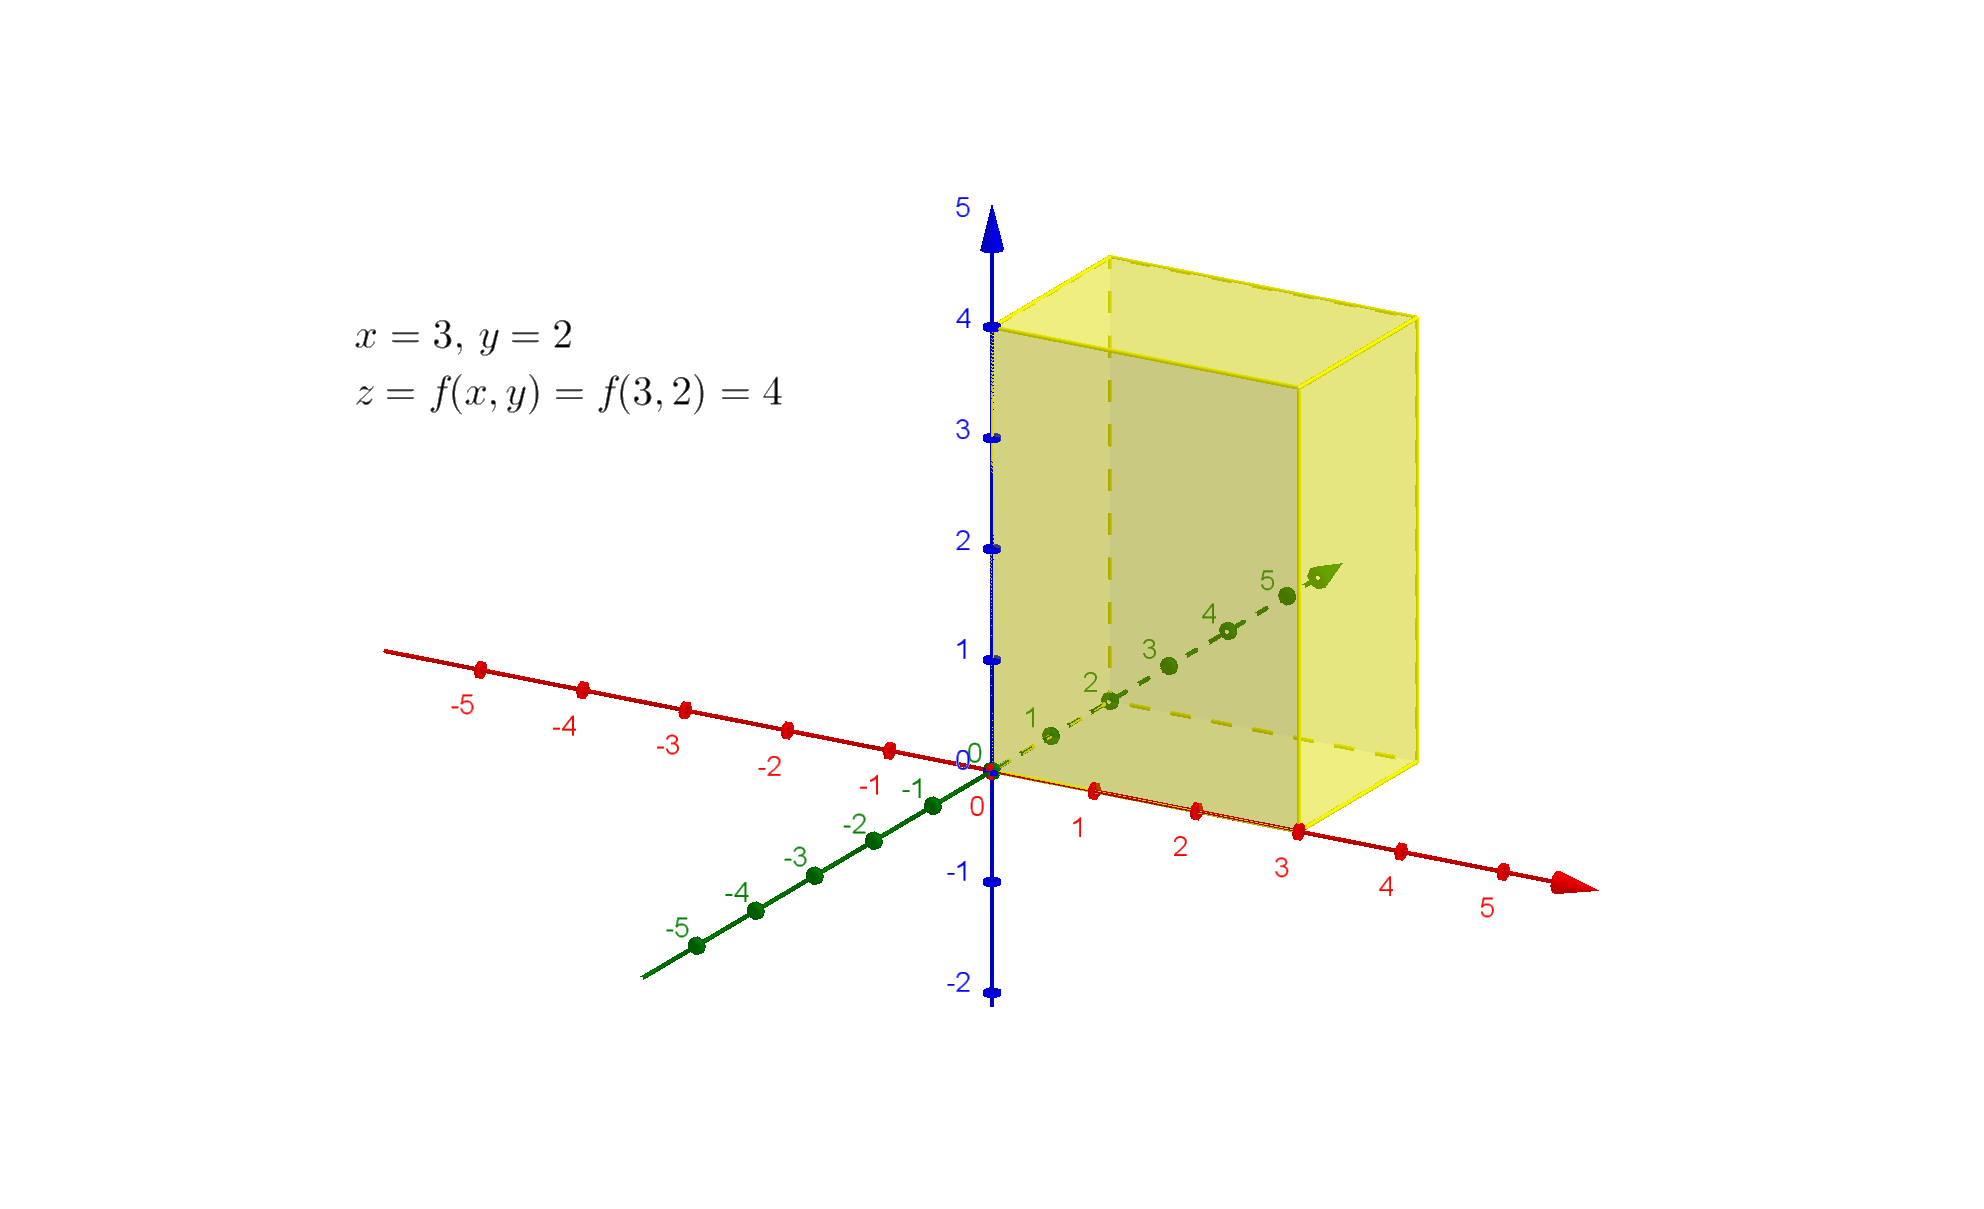
\includegraphics[width=\textwidth]{v01_a03_e01.png}
		\caption{Integrais duplas - Aula 3 - Exercício I}
		\label{v01_a03_e01}
	\end{figure}
	
	$z = 4;\; dz = dx dy$\newline\newline
	$v = \integral_0^3 \integral_0^2 z\, dz = \integral_0^3 \integral_0^2 4\, dy dx = 4\integral_0^3 dx \integral_0^2 dy = 4\integral_0^3 dx\, [y]_0^2 = 4\integral_0^3 dx\, [2 - 0] = 8\integral_0^3 dx = 8[x]_0^3 = 8[3 - 0] = 8 \cdot 3 = 24$\newline
	
	\item Exercício
	
	$R = [0, 3] \times [0,4]\\
	\integral \integral_R (8 - 2y) da$
	
	\begin{figure}[H]
		\centering
		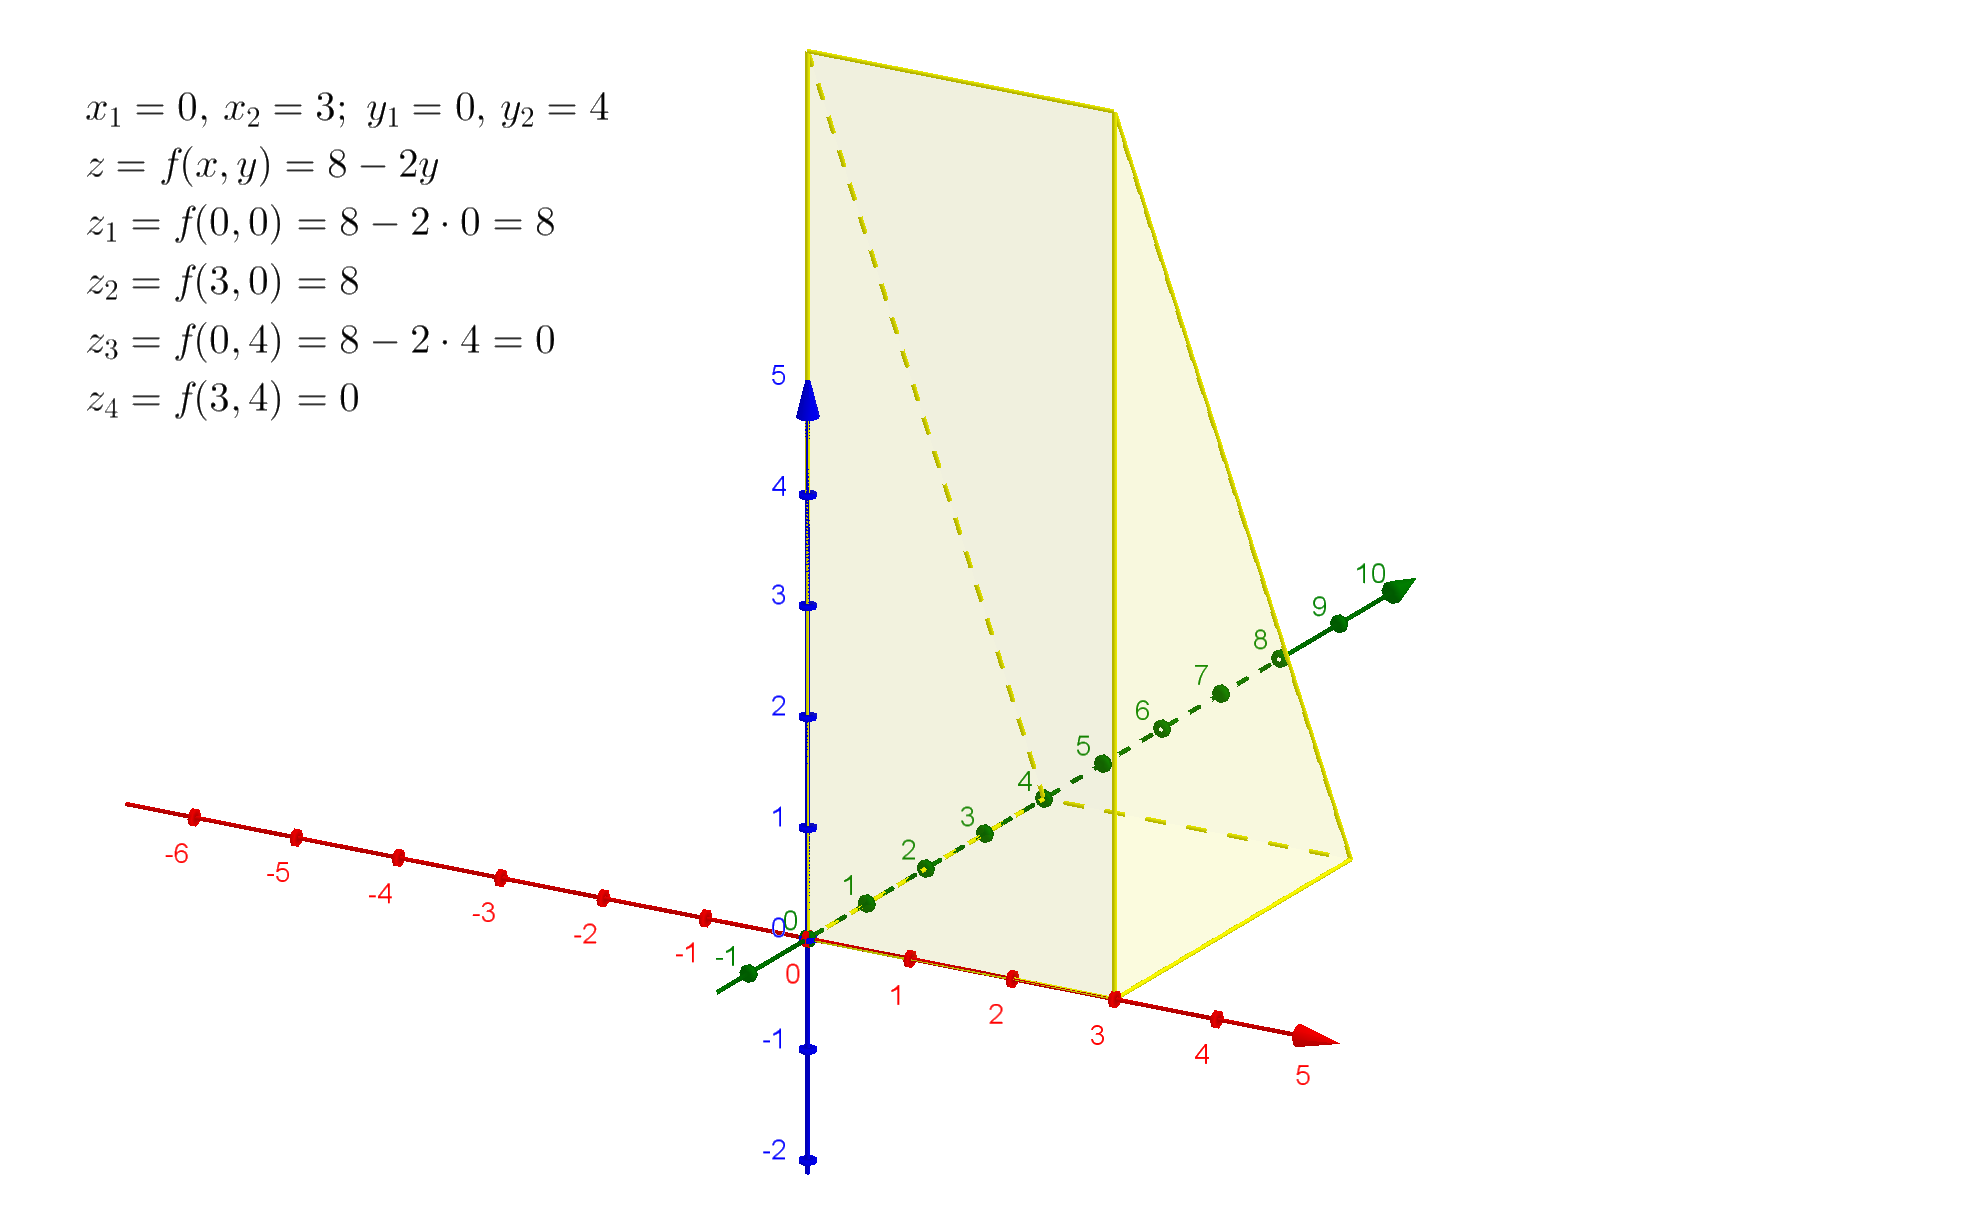
\includegraphics[width=\textwidth]{v01_a03_e02.png}
		\caption{Integrais duplas - Aula 3 - Exercício II}
		\label{v01_a03_e02}
	\end{figure}	
	
	$z = 8 - 2y;\; da = dz = dx dy$\newline\newline
	$v = \integral_0^3 \integral_0^4 z\,dz = \integral_0^3 \integral_0^4(8 - 2y)dx dy = \integral_0^3 dx \integral_0^4(8 - 2y) dy = \integral_0^3 dx \left(8\integral_0^4 dy - 2\integral_0^4 y\,dy\right) = \integral_0^3 dx\, 2\left(4\integral_0^4 dy - \integral_0^4 y\,dy\right) = 2\integral_0^3 dx \left[4y - \dfrac{y^2}{2}\right]_0^4 = 2\integral_0^3 dx \left[\dfrac{8y - y^2}{2}\right]_0^4 = \overstrike{2}\integral_0^3 dx\, \dfrac{1}{\overstrike{2}}[y(8 - y)]_0^4 = \integral_0^3 dx[4(8 - 4) \overstrike{- 0(8 - 0)}] = 16\integral_0^3 dx = 16[x]_0^3 = 16[3 - 0] = 48$
\end{enumerate}		
\section{Invertendo a ordem de integração - Aula 4}
	\begin{enumerate}
	\item Exercício
	
	\begin{equation*}
		z = f(x, y) = y\e^x;\; dz = dx dy	
	\end{equation*}
	\begin{align*}
		v = \int_2^4 \int_1^9 z\, dz = \int_2^4 \int_1^9 y\e^x\, dy dx = \int_2^4 \e^x\, dx \int_1^9 y\, dy = \int_2^4 \e^x\, dx \left[\dfrac{y^2}{2}\right]_1^9 =\\ \int_2^4 \e^x\, dx \dfrac{1}{2}\left[y^2\right]_1^9 = \dfrac{1}{2}\int_2^4 \e^x\, dx \left[9^2 - 1^2\right] = 40\int_2^4 \e^x\, dx = 40\left[\e^x\right]_2^4 = 40\left[\e^4 - \e^2\right] =\\ 40e^2\left(e^2 - 1\right)	
	\end{align*}
	
	\item Exercício
	
	\begin{equation*}
		z = f(x,y) = x^2y^3;\; dz = dx dy
	\end{equation*}
	
	\begin{figure}[htb]
		\caption{Integrais duplas - Aula 4 - Exercício II}
		\label{v04_a04_e02}
		\centering
		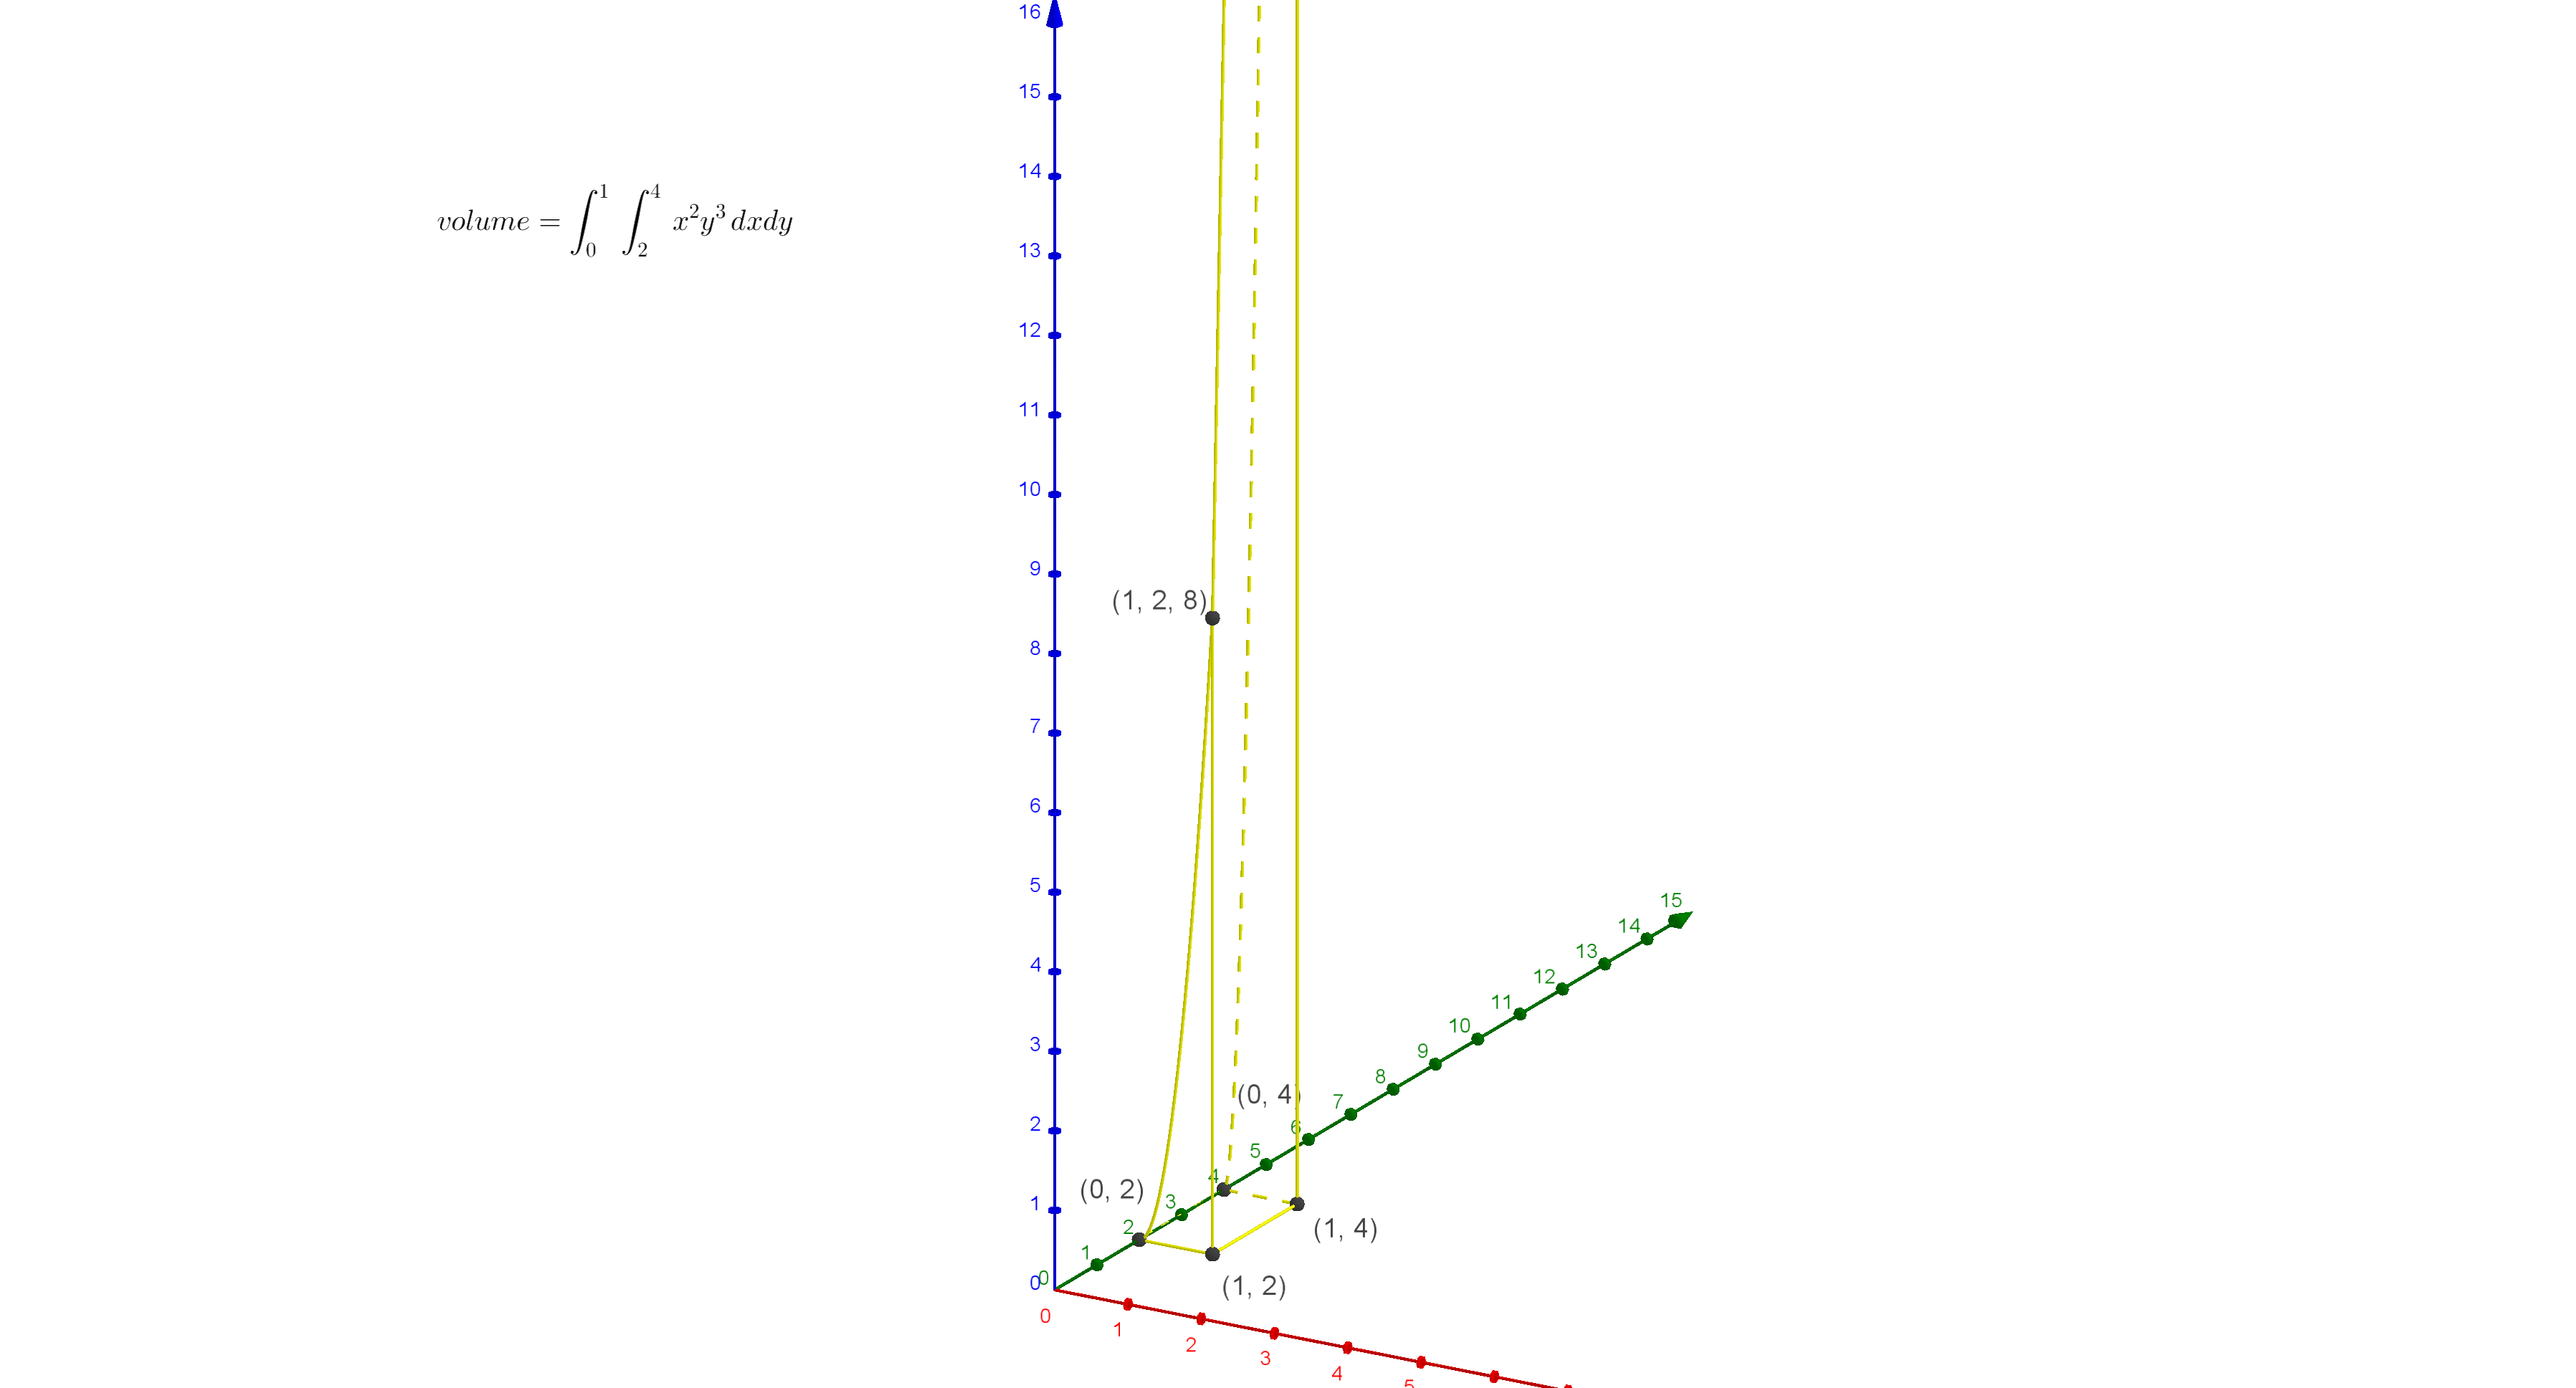
\includegraphics[width=0.5\textwidth]{v04_a04_e02.png}		
	\end{figure}
	
	\begin{align*}
		v = \int_0^1 \int_2^4 z\, dz = \int_0^1 \int_2^4 x^2y^3\, dx dy = \int_0^1 x^2\, dx \int_2^4 y^3\, dy = \int_0^1 x^2\, dx \left[\dfrac{y^4}{4}\right]_2^4 =\\ \dfrac{1}{4}\int_0^1 x^2\, dx \left[y^4\right]_2^4 = \dfrac{1}{4}\int_0^1 x^2\, dx \left[4^4 - 2^4\right] = \dfrac{1}{4}\int_0^1 x^2\, dx \left[2^8 - 2^4\right] =\\ \dfrac{1}{4}\int_0^1 x^2\, dx \left[2^4\left(2^4 - 1\right)\right] = \dfrac{1}{4}\int_0^1 x^2\, dx \left[16 \cdot 15\right] = 60\int_0^1 x^2\, dx = 60 \left[\dfrac{x^3}{3}\right]_0^1 = 20 \left[x^3\right]_0^1 =\\ 20 \left[1^3 - 0^3\right] = 20 \cdot 1 =  20
	\end{align*}
	
	\item Exercício
	
	\begin{equation*}
		\iint_R (x + 2y) da
	\end{equation*}
	
	$R$ = Região limitada pela parábola $y = x^2 + 1$ e as retas $x = -1$ e $x = 2$.
	
	\begin{equation*}
		z = f(x,y) = x + 2y;\; da = dz = dx dy
	\end{equation*}
	
	\begin{figure}[htb]
		\caption{Integrais duplas - Aula 4 - Exercício III}
		\label{v04_a04_e03}
		\centering
		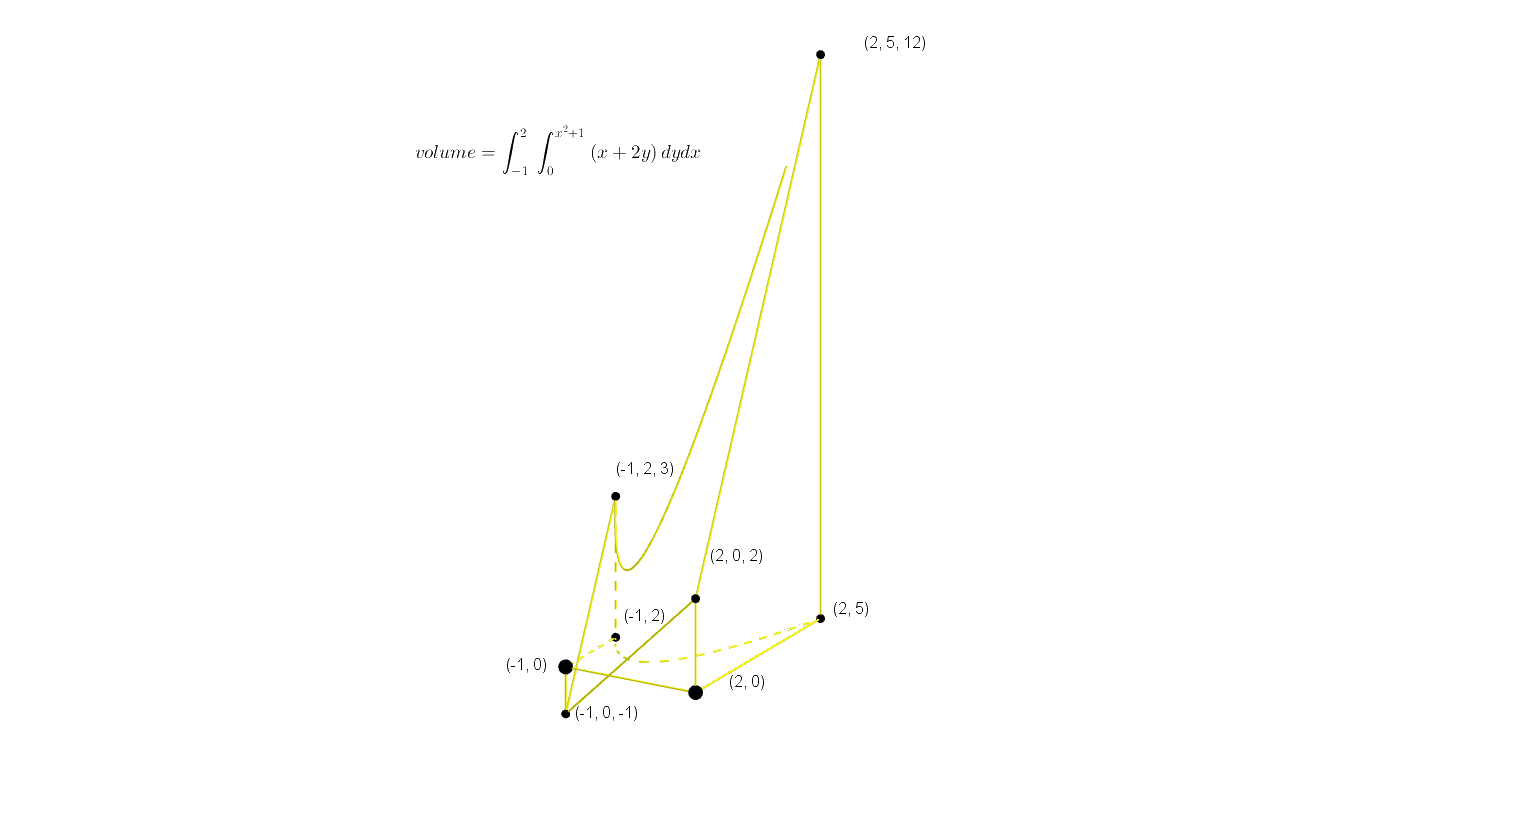
\includegraphics[width=0.5\textwidth]{v04_a04_e03.png}		
	\end{figure}
	
	\begin{align*}
		v = \int_{-1}^2 \int_0^{x^2 + 1} z\, dz = \int_{-1}^2 \int_0^{x^2 + 1} (x + 2y) dx dy =\\ \int_{-1}^2 dx \int_0^{x^2 + 1} (x + 2y) dy = \int_{-1}^2 dx \left(x\int_0^{x^2 + 1} dy + 2\int_0^{x^2 + 1} y\, dy\right) =\\ \int_{-1}^2 dx \left[xy + \overstrike{2}\dfrac{y^2}{\overstrike{2}}\right]_0^{x^2 + 1} = \int_{-1}^2 dx \left[y(x + y)\right]_0^{x^2 + 1} =\\ \int_{-1}^2 dx \left[\left(x^2 + 1\right)\left[x + \left(x^2 + 1\right)\right] \overstrike{- 0(x + 0)}\right] = \int_{-1}^2 dx \left[\left(x^2 + 1\right)\left(x^2 + x + 1\right)\right] =\\ \int_{-1}^2 dx \left(x^4 + x^3 + 2x^2 + x + 1\right) =\\ \int_{-1}^2 x^4\, dx + \int_{-1}^2 x^3\, dx + 2\int_{-1}^2 x^2\, dx + \int_{-1}^2 x\, dx + \int_{-1}^2 dx =\\ \left[\dfrac{x^5}{5} + \dfrac{x^4}{4} + 2\dfrac{x^3}{3} + \dfrac{x^2}{2} + x\right]_{-1}^2 = \left[\dfrac{12x^5 + 15x^4 + 40x^3 + 30x^2 + 60x}{60}\right]_{-1}^2 =\\ \dfrac{1}{60}\left[x\left(12x^4 + 15x^3 + 40x^2 + 30x + 60\right)\right]_{-1}^2 =\\ \dfrac{1}{60}\left[2\left(12\cdot2^4 + 15\cdot2^3 + 40\cdot2^2 + 30\cdot2 + 60\right) \right.\\\left.- (-1)\left(12(-1)^4 + 15(-1)^3 + 40(-1)^2 + 30(-1) + 60\right)\right] =\\ \dfrac{1}{60} [2(192 + 120 + 160 + 60 + 60) + (12 - 15 + 40 - 30 + 60)] = \dfrac{1}{60} (1184 + 67) =\\ \dfrac{1251}{60} = \frac{417}{20} = 20,85
	\end{align*}
\end{enumerate}		
\section{Cálculo de integrais duplas ou iteradas}
	\subsection{Aula 5}
		\begin{enumerate}
	\item Exercício
	
	\begin{equation*}
		f(x,y) = x^3;\; 0 \leq x \leq 2;\; x^2 \leq y \leq 4	
	\end{equation*}
	\begin{equation*}
		\iint_R f(x, y) dy dx
	\end{equation*}
	
	\begin{figure}[htb]
		\caption{Integrais duplas - Aula 5 - Exercício I}
		\label{v05_a05_e01}
		\centering
		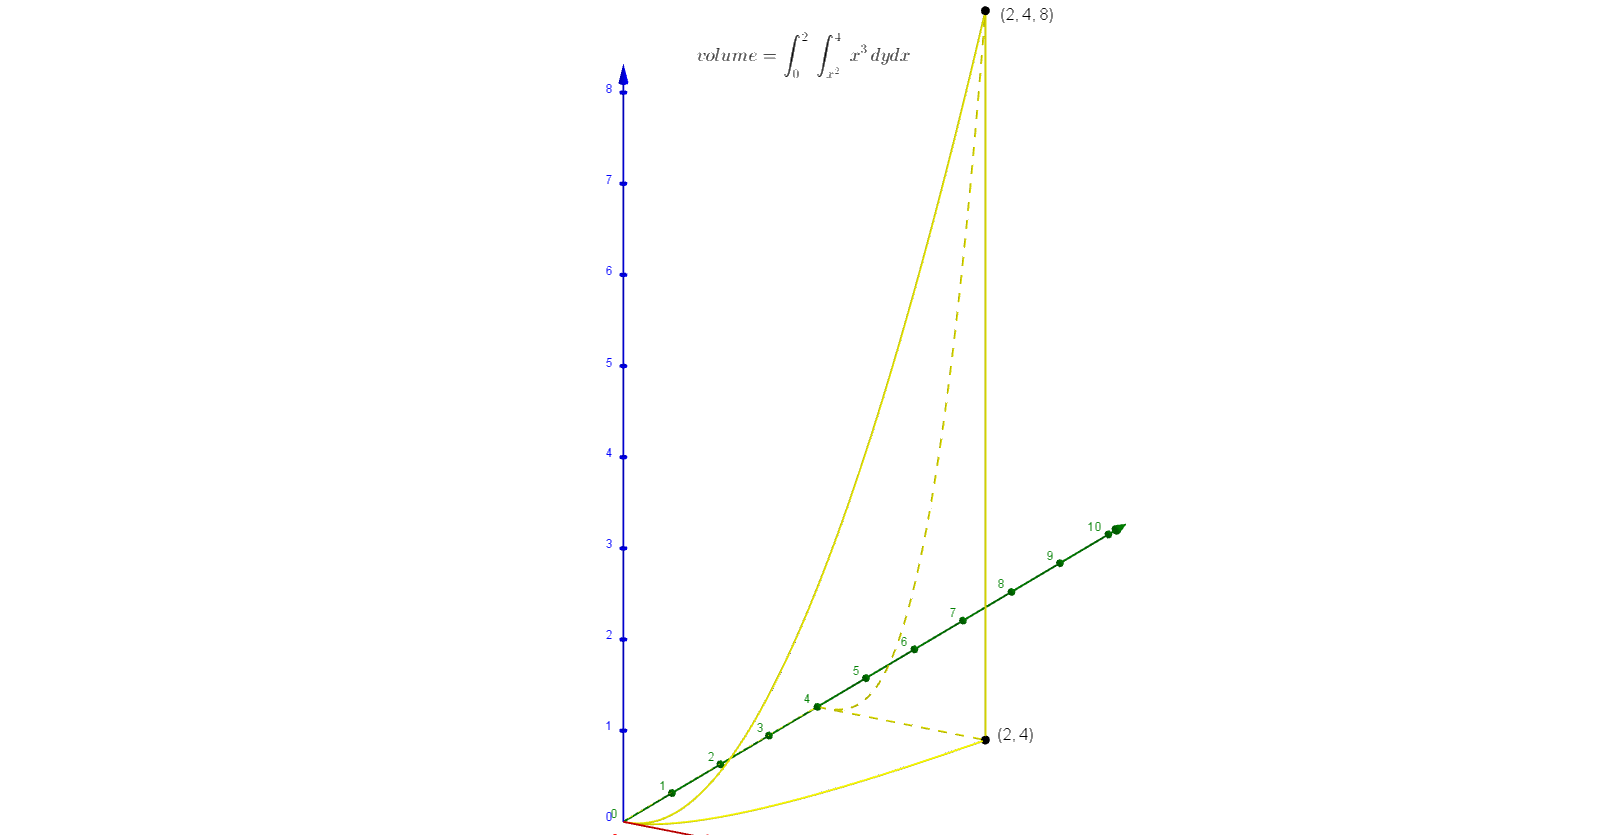
\includegraphics[width=0.5\textwidth]{v05_a05_e01.png}		
	\end{figure}
	
	\begin{gather*}
		v = \int_0^2 \int_{x^2}^4 x^3\, dy dx = \int_0^2 x^3\, dx \int_{x^2}^4 dy = \int_0^2 x^3\, dx\, [y]_{x^2}^4 = \int_0^2 x^3\, dx\, \left[4 - x^2\right] =\\ 4\int_0^2 x^3\, dx - \int_0^2 x^5\, dx = \left[\overstrike{4}\dfrac{x^4}{\overstrike{4}} - \frac{x^6}{6}\right]_0^2 = \left[\dfrac{6x^4 - x^6}{6}\right]_0^2 = \frac{1}{6}\left[x^4\left(6 - x^2\right)\right]_0^2 =\\ \frac{1}{6}\left[2^4\left(6 - 2^2\right) - \overstrike{0^4\left(6 - 0^2\right)}\right] = \dfrac{1}{6}(16\cdot2) = \dfrac{32}{6} = \dfrac{16}{3} = 5,2
	\end{gather*}
	
	\item Exercício
	
	\begin{equation*}
		f(x,y) = x^2y;\; 1 \leq x \leq 3;\; x \leq y \leq 2x + 1
	\end{equation*}
	\begin{equation*}
		\iint_R f(x, y) dy dx
	\end{equation*}
	
	\begin{figure}[htb]
		\caption{Integrais duplas - Aula 5 - Exercício II}
		\label{v05_a05_e02}
		\centering
		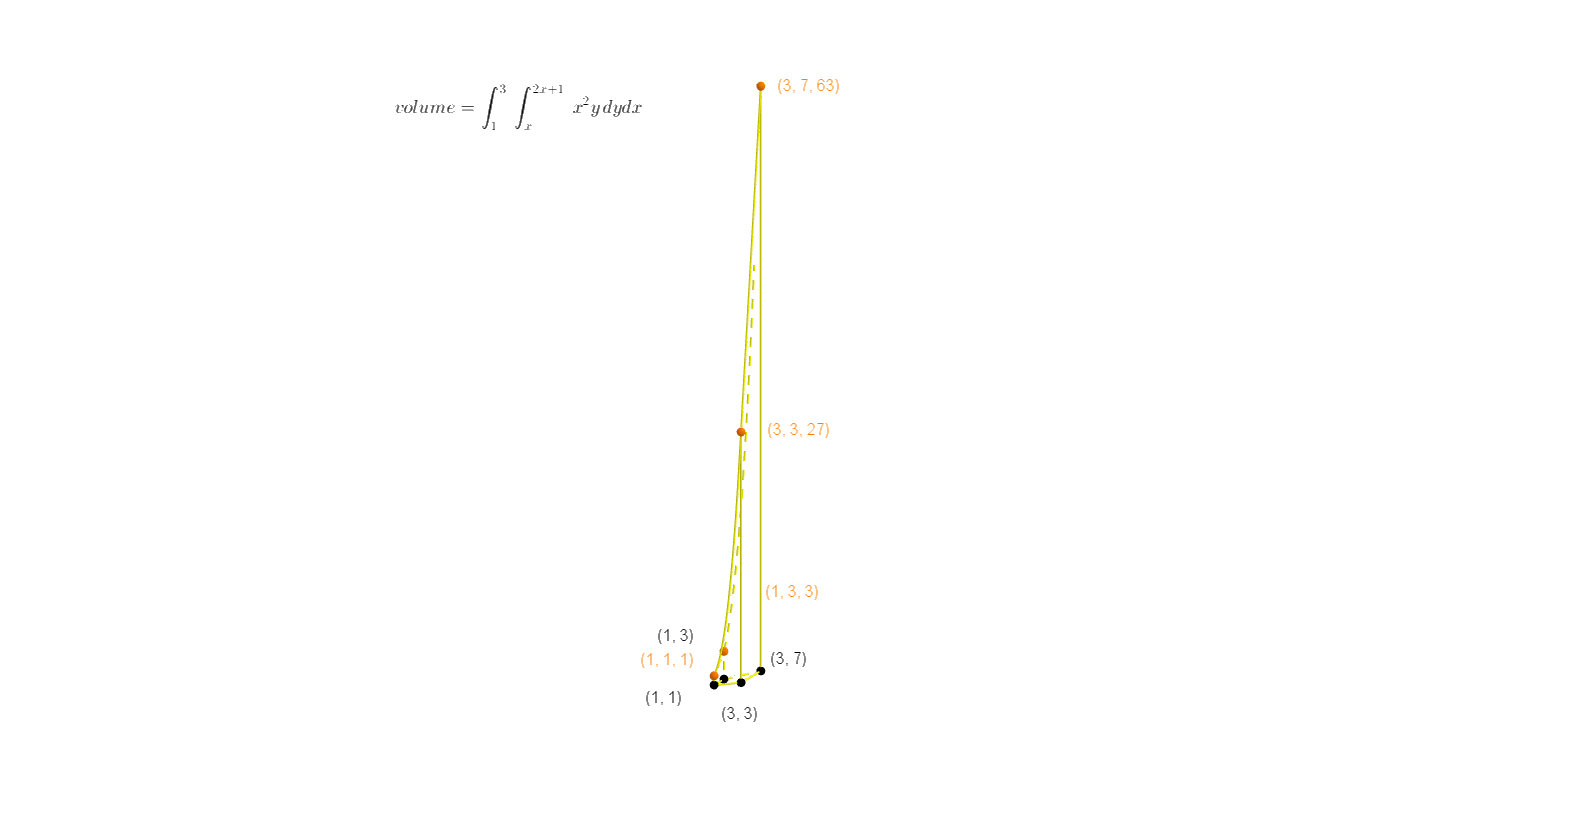
\includegraphics[width=0.5\textwidth]{v05_a05_e02.png}		
	\end{figure}
	
	\begin{gather*}
		v = \int_1^3 \int_x^{2x + 1} x^2y\, dy dx = \int_1^3 x^2\, dx \int_x^{2x + 1} y\, dy =  \int_1^3 x^2\, dx \left[\dfrac{y^2}{2}\right]_x^{2x + 1} =\\  \int_1^3 x^2\, dx \dfrac{1}{2}\left[(2x + 1)^2 - (x)^2\right] = \dfrac{1}{2}\int_1^3 x^2\, dx \left(3x^2 + 4x + 1\right) =\\ \dfrac{3}{2}\int_1^3 x^4\, dx + 2\int_1^3 x^3\, dx + \dfrac{1}{2}\int_1^3 x^2\, dx = \left[\dfrac{3}{2}\dfrac{x^5}{5} + 2\frac{x^4}{4} + \dfrac{1}{2}\dfrac{x^3}{3}\right]_1^3 = \left[\dfrac{3x^5}{10} + \dfrac{x^4}{2} + \frac{x^3}{6}\right]_1^3 =\\ \left[\dfrac{18x^5 + 30x^4 + 10x^3}{60}\right]_1^3 = \left[\dfrac{2x^3\left(9x^2 + 15x + 5\right)}{60}\right]_1^3 =\\ \dfrac{1}{30}\left[x^3\left(9x^2 + 15x + 5\right)\right]_1^3 = \dfrac{1}{30}\left[3^3\left(9\cdot3^2 + 15\cdot3 + 5\right) - 1^3\left(9\cdot1^2 + 15\cdot1 + 5\right)\right] =\\ \dfrac{1}{30}\left[27(81 + 45 + 5) - (9 + 15 + 5)\right] = \dfrac{1}{30}\left[27\cdot131 - 29\right] = \frac{3508}{30} = 116,9\overline{3}	
	\end{gather*}
\end{enumerate}		
	\subsection{Aula 6}
		\begin{enumerate}
	\item Exercício
	
	$f(x,y) = 1;\; 0 \leq x \leq 1;\; 1 \leq y \leq \e^x$\newline
	$\iintegral_R f(x, y) dy dx$\newline\newline
	$v = \integral_0^1 \integral_1^{\e^x} dy dx = \integral_0^1 dx\, [y]_1^{\e^x} = \integral_0^1 dx\, \left(\e^x - 1\right) = \left[\e^x - x\right]_0^1 = \e^1 - 1 - \left(\e^0 - 0\right) = \e - 1 - 1 = \e - 2$\newline
	
	\item Exercício
	
	$f(x,y) = x;\; 0 \leq x \leq 1;\; 1 \leq y \leq \e^{x^2}$\newline
	$\iintegral_R f(x, y) dy dx$\newline\newline
	$v = \integral_0^1 \integral_1^{\e^{x^2}} x\,	dx dy = \integral_0^1 x\,	dx \integral_1^{\e^{x^2}} dy = \integral_0^1 x\,	dx\, [y]_1^{\e^{x^2}} = \integral_0^1 x\,	dx\, \left(\e^{x^2} - 1\right) = \integral_0^1 x\e^{x^2}\,	dx - \integral_0^1 x\,	dx = \integral_0^1 \e^u\, \dfrac{du}{2} - \integral_0^1 x\,	dx = \dfrac{1}{2}\integral_0^1 \e^u\, du - \integral_0^1 x\,	dx = \left[\dfrac{1}{2}e^u - \dfrac{x^2}{2}\right]_0^1 = \left[\dfrac{e^{x^2} - x^2}{2}\right]_0^1 = \dfrac{1}{2} \left[e^{x^2} - x^2\right]_0^1 = \dfrac{1}{2} \left[e^{1^2} - 1^2 - \left(e^{0^2} - 0^2\right)\right] = \dfrac{1}{2}(\e - 1 - 1) = \dfrac{\e - 2}{2}$\newline\newline
	$u = x^2 ;\; \dfrac{du}{2} = x\, dx$
	
	\item Exercício
	
	$f(x,y) = 2xy;\; 0 \leq y \leq 1;\; y^2 \leq x \leq y$\newline
	$\iintegral_R f(x, y) dx dy$\newline\newline
	$v = \integral_0^1 \integral_{y^2}^y 2xy\, dx dy = 2\integral_0^1 y\, dy \integral_{y^2}^y x\, dx = 2\integral_0^1 y\, dy\, \left[\dfrac{x^2}{2}\right]_{y^2}^y = \overstrike{2}\integral_0^1 y\, dy\, \dfrac{1}{\overstrike{2}}\left[x^2\right]_{y^2}^y = \integral_0^1 y\, dy\, \left(y^2 - y^4\right) = \integral_0^1 \left(y^3 - y^5\right) dy = \left[\frac{y^4}{4} - \frac{y^6}{6}\right]_0^1 = \left[\dfrac{6y^4 - 4y^6}{24}\right]_0^1 = \left[\dfrac{2y^4\left(3 - 2y^2\right)}{24}\right]_0^1 = \dfrac{1}{12}\left[1^4\left(3 - 2\cdot1^2\right) \overstrike{- 0^4\left(3 - 2\cdot0^2\right)}\right] = \dfrac{1}{12} = 0,08\overline{3}$
\end{enumerate}		
	\subsection{Aula 7}
		\begin{enumerate}
	\item Exercício
	
	\begin{equation*}
		f(x,y) = \dfrac{1}{x + y};\; 1 \leq y \leq \e;\; 0 \leq x \leq y	
	\end{equation*}
	\begin{equation*}
		\iint_R f(x, y) dx dy
	\end{equation*}
	\begin{gather*}
		v = \int_1^{\e} \int_0^y \dfrac{1}{x + y}\, dx dy = \int_1^{\e} dy \int_0^y (x + y)^{-1}\, dx = \int_1^{\e} dy \int_0^y u^{-1}\, du =\\ \int_1^{\e} dy \int_0^y\, \left[\ln |u|\right]_0^y = \int_1^{\e} dy \int_0^y\, \left[\ln |x + y|\right]_0^y = \int_1^{\e} dy \int_0^y\, \left(\ln |y + y| - \ln |0 + y|\right) =\\ \int_1^{\e} dy \int_0^y\, \left(\ln |2y| - \ln |y|\right) = \int_1^{\e} dy \int_0^y\, \left(\ln |2| \overstrike{+ \ln |y| - \ln |y|}\right) = \ln |2|\int_1^{\e} dy =\\ \ln |2|[y]_1^{\e} = \ln |2|(\e - 1)
	\end{gather*}
	\begin{equation*}
		u = x + y;\; du = (1 + 0)dx = dx
	\end{equation*}
\end{enumerate}		
	\section{Cálculo de área - Aula 8}
		\begin{enumerate}
	\item Exercício
	
	\begin{figure}[htb]
		\caption{Integrais duplas - Aula 8 - Exercício I}
		\label{v08_a08_e01}
		\centering
		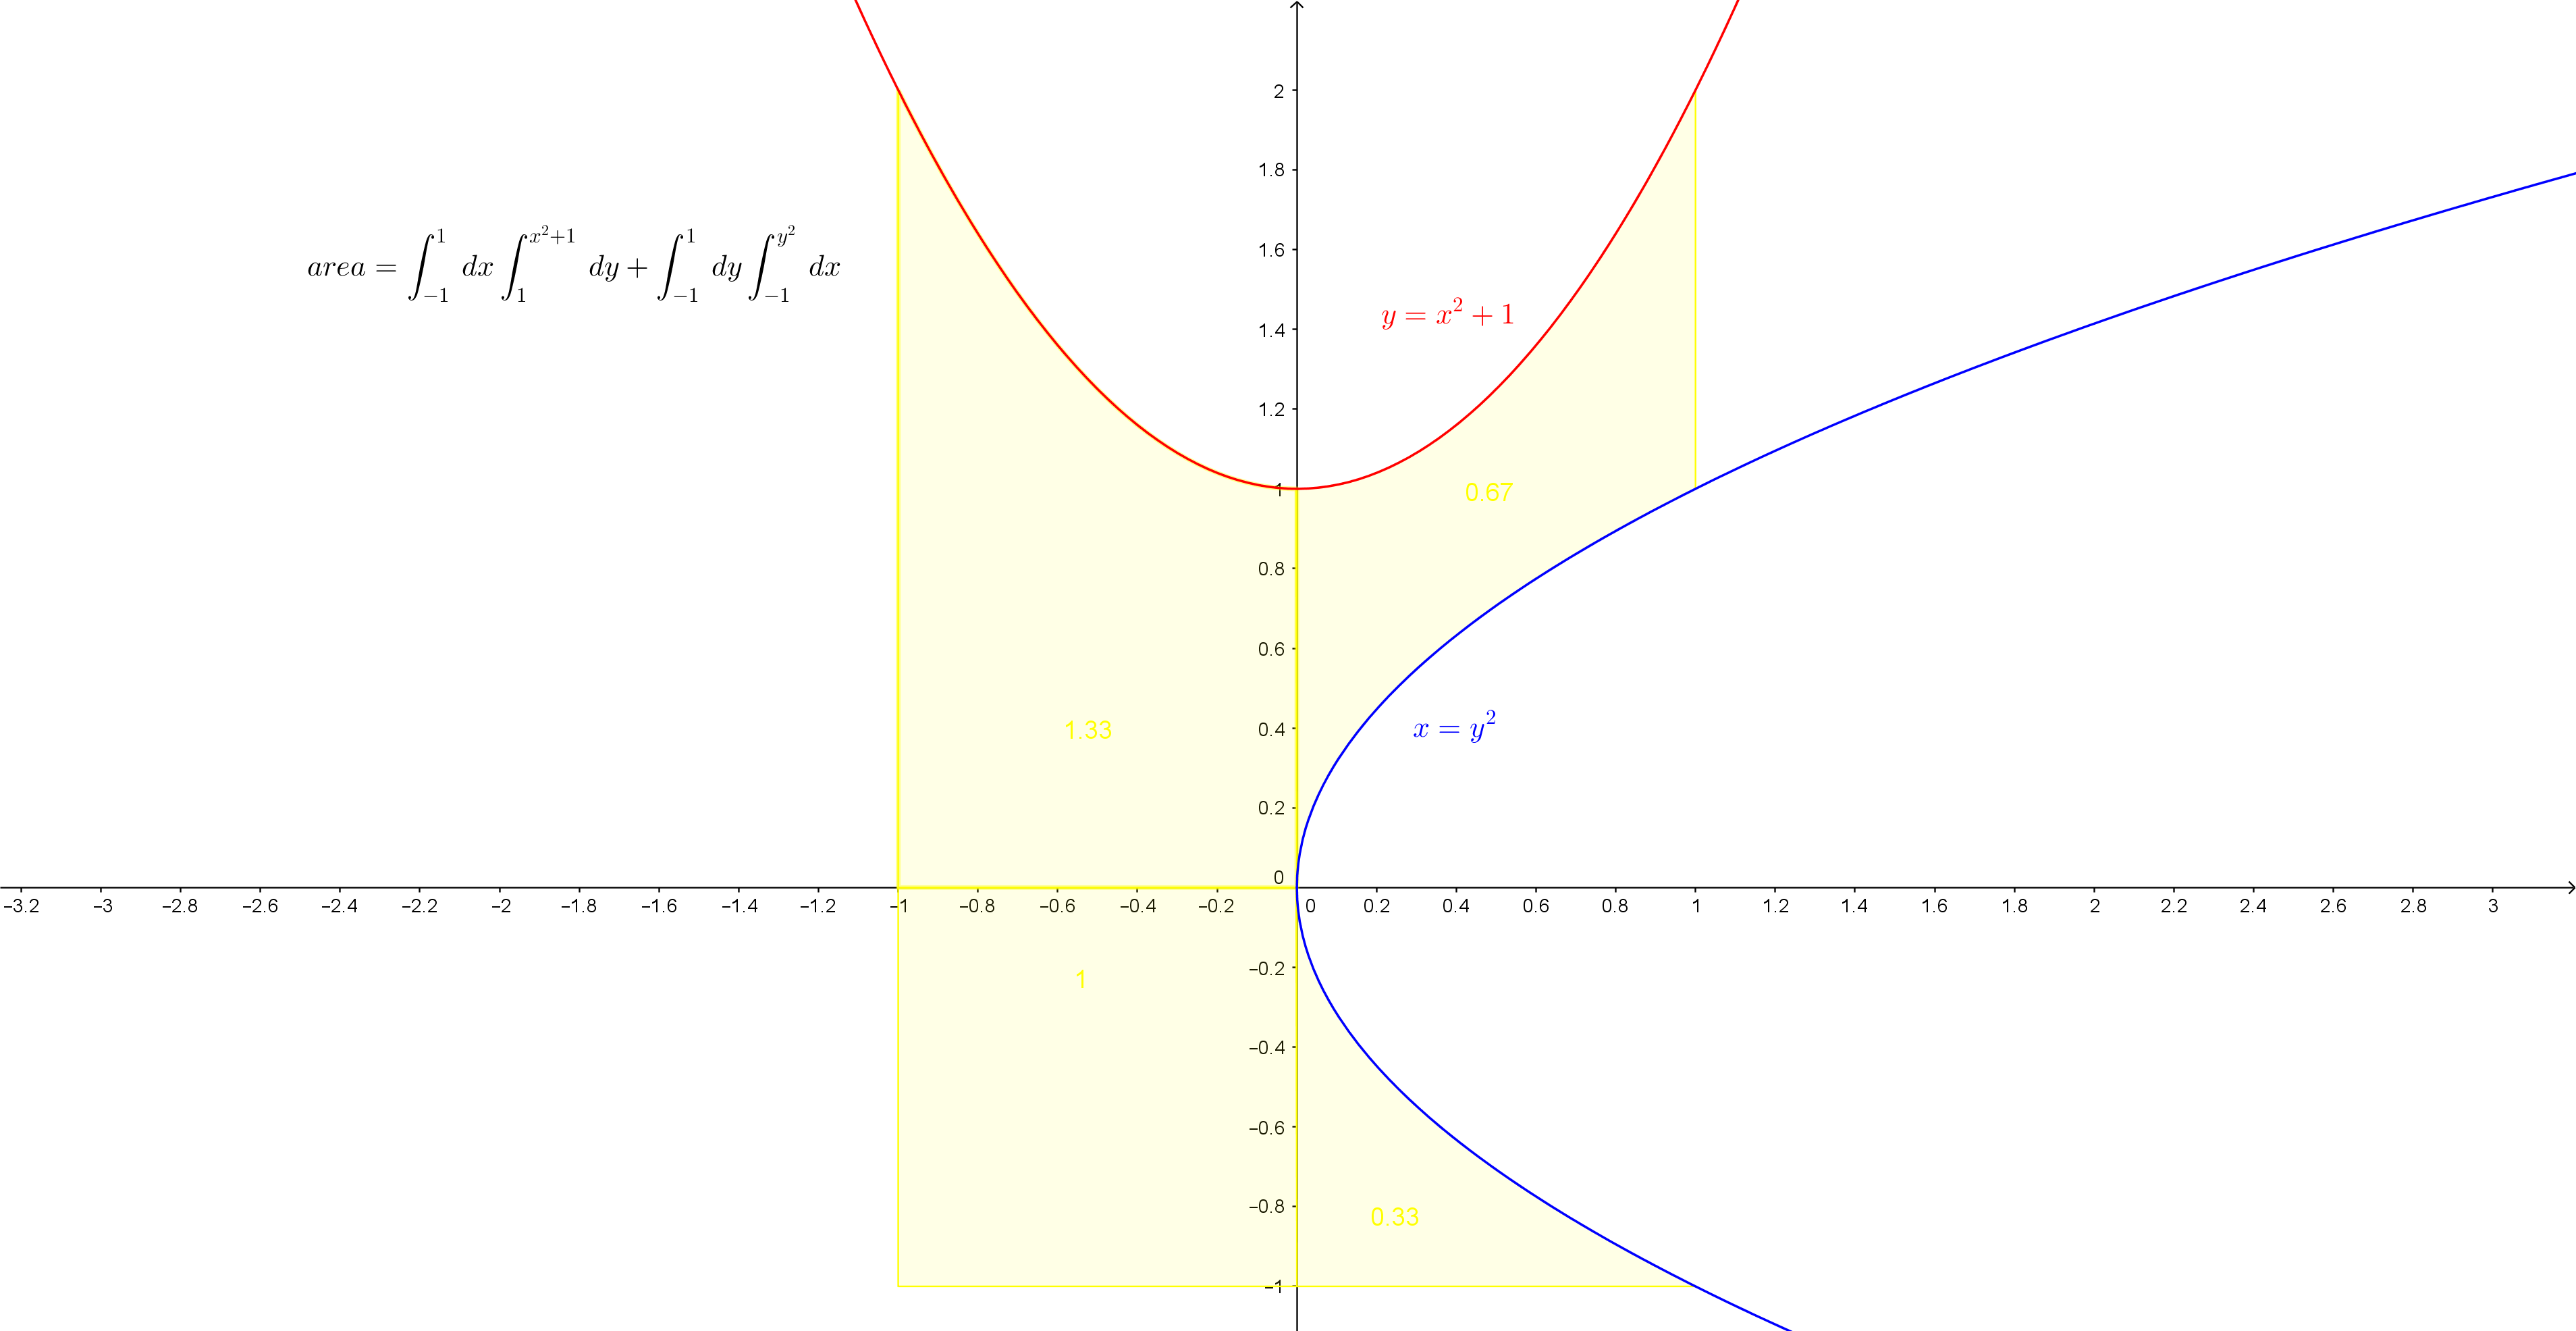
\includegraphics[width=0.5\textwidth]{v08_a08_e01.png}		
	\end{figure}
	
	\begin{align*}
		a = \int_{-1}^0 dx \int_0^{x^2 + 1} dy + \int_{-1}^0 dx \int_{-1}^0 dy + \int_0^{y^2} dx \int_{-1}^0 dy + \int_0^1 dx \int_{\sqrt{x}}^{x^2 + 1} =\\ \int_{-1}^0 dx\left(\int_0^{x^2 + 1} dy + \int_{-1}^0 dy\right)  + \int_0^{y^2} dx \int_{-1}^0 dy + \int_0^1 dx \int_{\sqrt{x}}^{x^2 + 1} =\\ \int_{-1}^0 dx \left([y]_0^{x^2 + 1} + [y]_{-1}^0\right)  + \int_{-1}^0 dy\, [x]_0^{y^2} + \int_0^1 dx\, [y]_{\sqrt{x}}^{x^2 + 1} =\\ \int_{-1}^0 dx\, \left(x^2 + 1 + 1\right) + \int_{-1}^0 dy\, y^2 + \int_0^1 dx\, \left(x^2 + 1 - \sqrt{x}\right) =\\ \int_{-1}^0 \left(x^2 + 2\right) dx + \int_{-1}^0 y^2\, dy + \int_0^1 \left(x^2 - x^{\frac{1}{2}} + 1\right) dx =\\ \left[\dfrac{x^3}{3} + 2x\right]_{-1}^0 + \left[\dfrac{y^3}{3}\right]_{-1}^0 + \left[\dfrac{x^3}{3} - \dfrac{x^{\frac{3}{2}}}{\left(\dfrac{3}{2}\right)} + x\right]_0^1 =\\ \left[\dfrac{x^3 + 6x}{3}\right]_{-1}^0 + \dfrac{1}{3}\left[y^3\right]_{-1}^0 + \left[\dfrac{x^3}{3} - \dfrac{2\sqrt{x^3}}{3} + x\right]_0^1 =\\ \dfrac{1}{3}\left[x\left(x^2 + 6\right)\right]_{-1}^0 + \dfrac{1}{3}\left[\overstrike{0^3} - (-1)^3\right] + \left[\dfrac{x^3 - 2\sqrt{x^3} + 3x}{3}\right]_0^1 =\\ \dfrac{1}{3}\left[\overstrike{0\left(0^2 + 6\right)} - (-1)\left((-1)^2 + 6\right)\right] + \dfrac{1}{3} + \dfrac{1}{3}\left[x^3 - 2\sqrt{x^3} + 3x\right]_0^1 =\\ \dfrac{7}{3} + \dfrac{1}{3} + \dfrac{1}{3}\left[1^3 - 2\sqrt{1^3} + 3\cdot1 \overstrike{- \left(0^3 - 2\sqrt{0^3} + 3\cdot0\right)}\right] = \dfrac{7}{3} + \dfrac{1}{3} + \dfrac{2}{3} =\\ \dfrac{7 + 1 + 2}{3} = \dfrac{10}{3} = 3,\overline{3}	
	\end{align*}	
	\begin{align*}
		a = \int_{-1}^1 dx \int_1^{x^2 + 1} dy + \int_{-1}^{y^2} dx \int_{-1}^1 dy = \int_{-1}^1 dx\, [y]_1^{x^2 + 1} + \int_{-1}^1 dy\, [x]_{-1}^{y^2} =\\ \int_{-1}^1 dx\, \left(x^2 \overstrike{+ 1 - 1}\right) + \int_{-1}^1 dy\, \left(y^2 + 1\right) = \left[\dfrac{x^3}{3}\right]_{-1}^1 + \left[\dfrac{y^3}{3} + y\right]_{-1}^1 =\\ \dfrac{1}{3}\left[x^3\right]_{-1}^1 + \dfrac{1}{3}\left[y\left(y^2 + 3\right)\right]_{-1}^1 =\\ \dfrac{1}{3}\left(\left[1^3 - (-1)^3\right] + \left[1\left(1^2 + 3\right) - (-1)\left((-1)^2 + 3\right)\right]\right)\dfrac{1}{3}(2 + 4 + 4) = \frac{10}{3} = 3,\overline{3}
	\end{align*}
\end{enumerate}		
	\section{Cálculo de volume}
		\subsection{Aula 9}
			\begin{enumerate}
	\item Exercício
	
	Esboçe a região de integração e o sólido cujo volume é dado pela integral abaixo: 
	$$\integral_0^1 \integral_0^1 \left(4 - x - 2y\right)\, dx dy$$
	
	\begin{figure}[H]
		\centering
		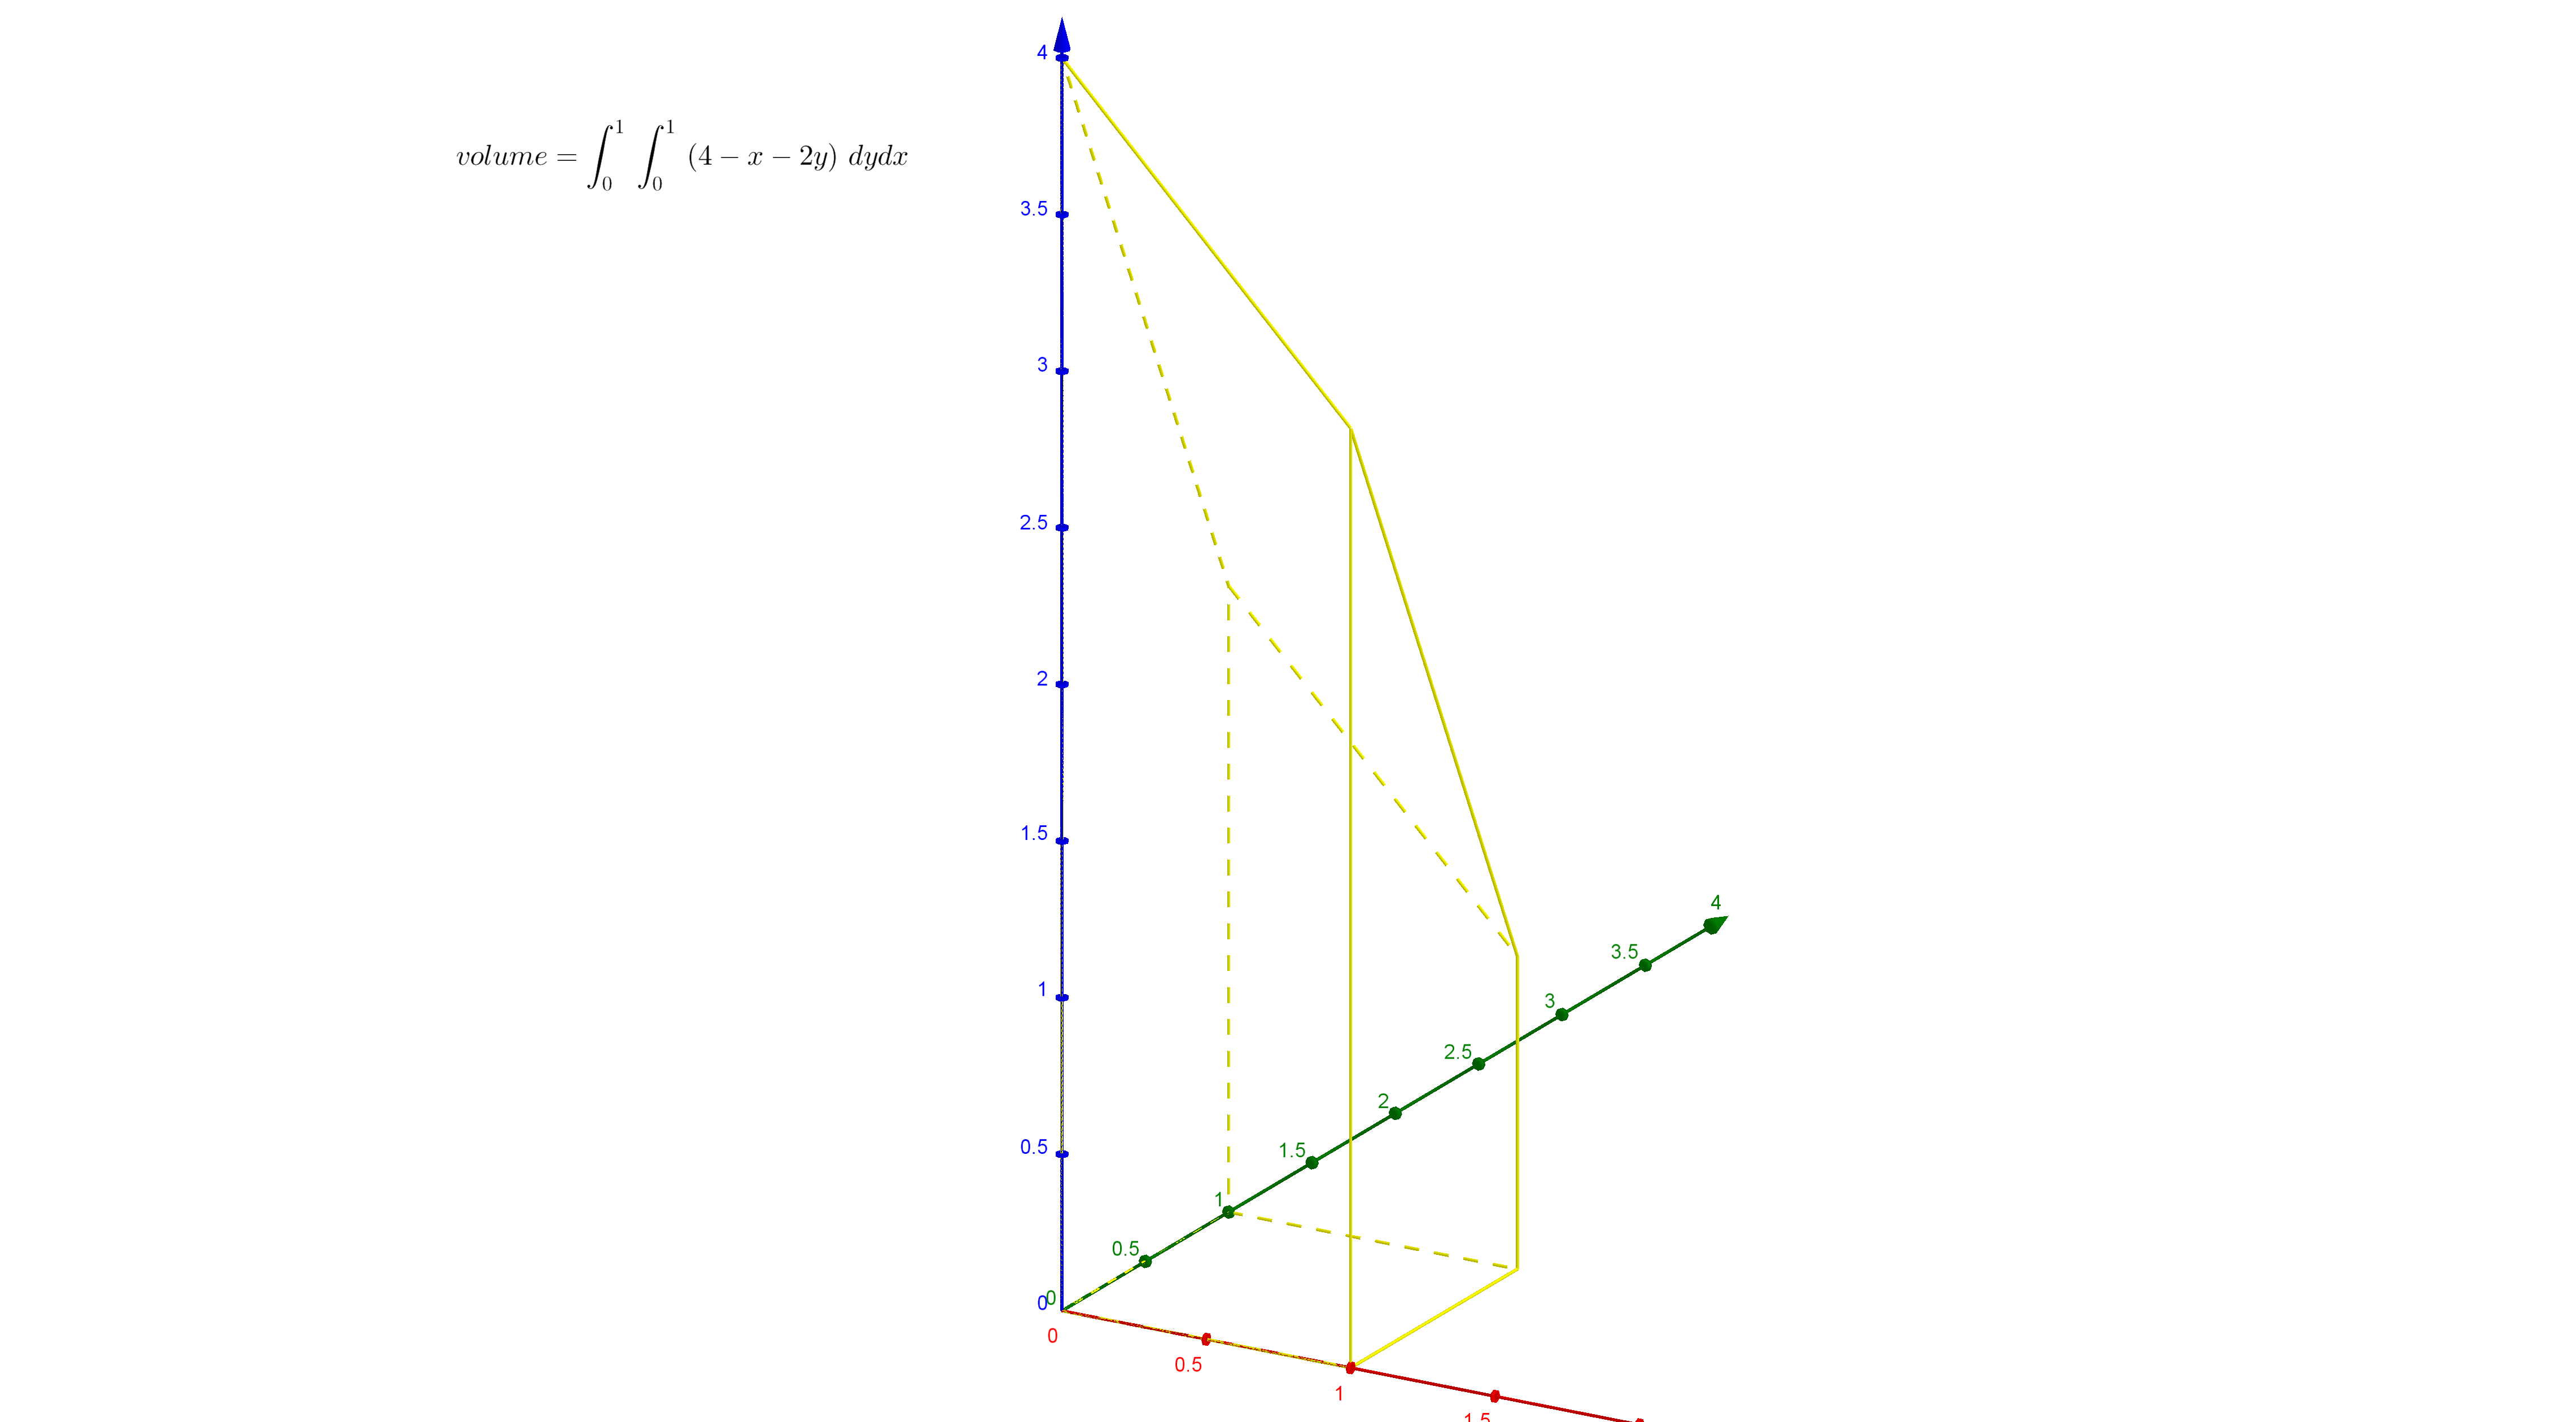
\includegraphics[width=\textwidth]{v09_a09_e01.png}
		\caption{Integrais duplas - Aula 9 - Exercício I}
		\label{v09_a09_e01}
	\end{figure}
	
	$v = \integral_0^1 \integral_0^1 \left(4 - x - 2y\right)\, dx dy = \integral_0^1 dx \left(4\integral_0^1 dy - x\integral_0^1 dy - 2\integral_0^1 y\, dy\right) = 4\integral_0^1 dx \integral_0^1 dy - \integral_0^1 x\, dx \integral_0^1 dy - 2\integral_0^1 dx \integral_0^1 y\, dy = 4[x]_0^1 [y]_0^1 - \left[\dfrac{x^2}{2}\right]_0^1 [y]_0^1 - 2[x]_0^1 \left[\dfrac{y^2}{2}\right]_0^1 = 4 - \dfrac{1}{2} - \overstrike{2}\dfrac{1}{\overstrike{2}} = \frac{8 - 1 - 2}{2} = \dfrac{5}{2} = 2,5$
	
	
\end{enumerate}		
		\subsection{Aula 10}
			\begin{enumerate}
	\item Exercício
	
	Calcule o volume do sólido limitado pelos planos:
	\begin{equation*}
		x = 0,\, y = 0,\, z = 0 \textrm{ e } 6x + 2y + 3z = 6
	\end{equation*}
	
	\begin{figure}[htb]
		\caption{Integrais duplas - Aula 10 - Exercício I}
		\label{v10_a10_e01}
		\centering
		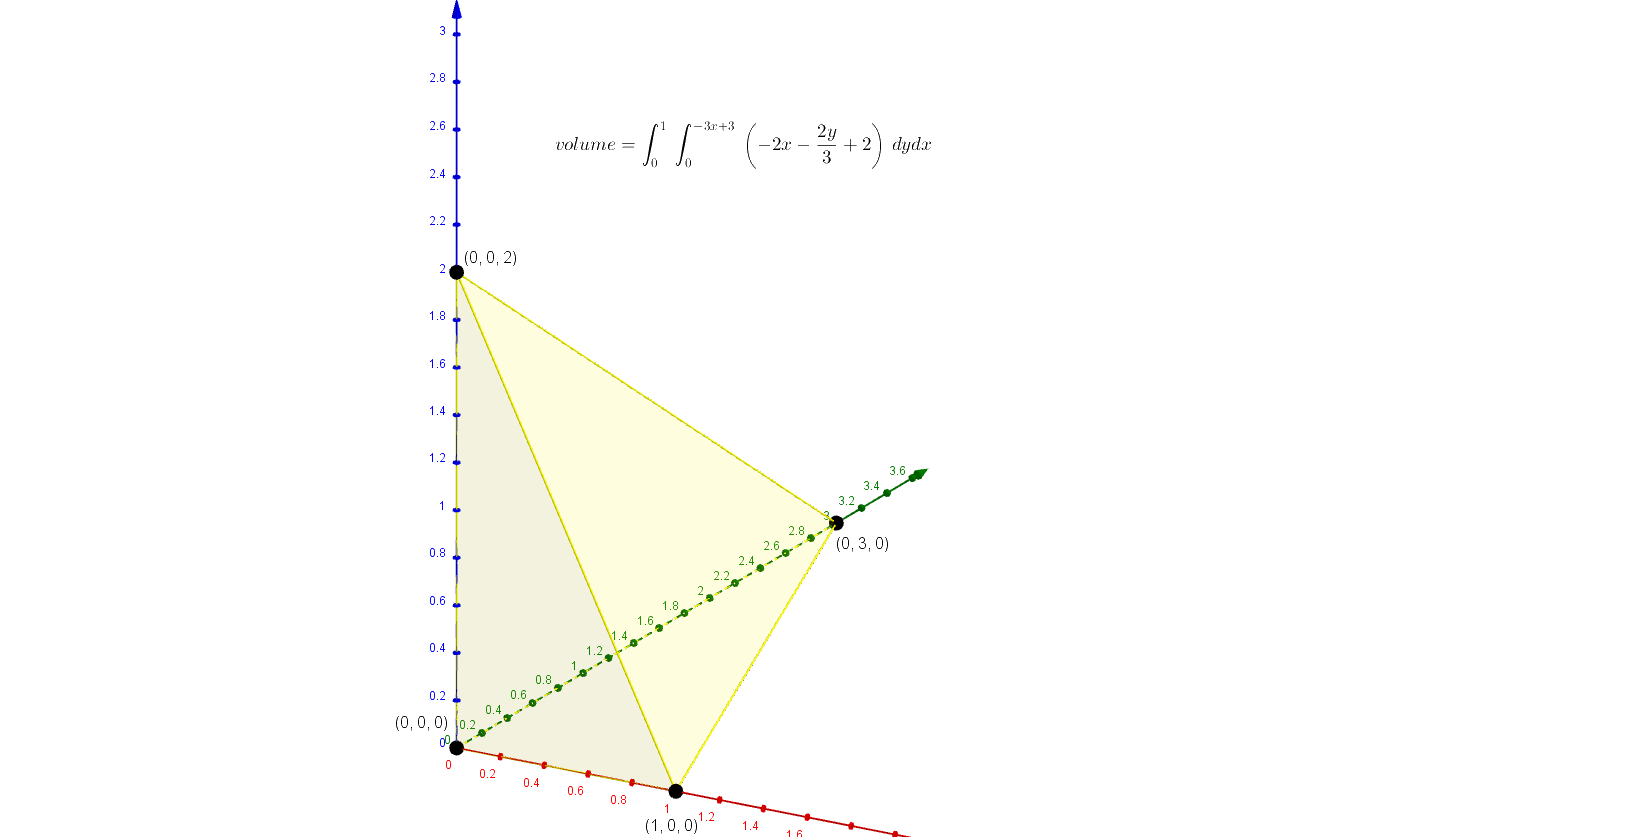
\includegraphics[width=0.5\textwidth]{v10_a10_e01.png}		
	\end{figure}
	
	\begin{equation*}
		P_1 = (0, 0 , 0)	
	\end{equation*}
	\begin{equation*}
		6x = -2y - 3z + 6 \Rightarrow x = \dfrac{-2y - 3z + 6}{6} = \dfrac{-2\cdot0 - 3\cdot0 + 6}{6} = \dfrac{6}{6} = 1 \Rightarrow P_2 = (1,0,0)
	\end{equation*}
	\begin{equation*}
		2y = -6x - 3z + 6 \Rightarrow y = \dfrac{-6x - 3z + 6}{2} = \dfrac{-6\cdot0 - 3\cdot0 + 6}{2} = \dfrac{6}{2} = 3 \Rightarrow P_3 = (0,3,0)
	\end{equation*}
	\begin{equation*}
		3z = -6x - 2y + 6 \Rightarrow z = \dfrac{-6x - 2y + 6}{3} = \dfrac{-6\cdot0 - 2\cdot0 + 6}{3} = \dfrac{6}{3} = 2 \Rightarrow P_4 = (0,0,2)
	\end{equation*}
	\begin{equation*}
		x = 0, x = 1
	\end{equation*}
	\begin{equation*}
		y = 0,\, y = \dfrac{-6x - 3z + 6}{2} = \dfrac{-6x - 3\cdot0 + 6}{2} = -3x + 3
	\end{equation*}
	\begin{equation*}
		z = \dfrac{-6x - 2y + 6}{3} = -2x - \dfrac{2y}{3} + 2
	\end{equation*}
	\begin{gather*}
		v = \int_0^1 \int_0^{-3x + 3} \left(-2x - \dfrac{2y}{3} + 2\right)\, dx dy = \int_0^1 dx \int_0^{-3x + 3} \left(-2x - \dfrac{2y}{3} + 2\right)\, dy =\\ \int_0^1 dx\, \left[-2xy - \dfrac{\overstrike{2}}{3}\dfrac{y^2}{\overstrike{2}} + 2y\right]_0^{-3x + 3} = \int_0^1 dx\, \dfrac{1}{3}\left[-6xy - y^2 + 6y\right]_0^{-3x + 3} =\\ \dfrac{1}{3}\int_0^1 dx\, \left[-y(6x + y - 6)\right]_0^{-3x + 3} =\\ \dfrac{1}{3}\int_0^1 dx\, \left[-(-3x + 3)(6x + (-3x + 3) - 6) \overstrike{+ 0(6x + 0 - 6)}\right] =\\ \dfrac{1}{3}\int_0^1 dx\, \left[(3x-3)(3x - 3)\right] = \dfrac{1}{3}\int_0^1 \left(9x^2 - 18x + 9\right) dx = \dfrac{1}{3}\left[9\dfrac{x^3}{3} - 18 \dfrac{x^2}{2} + 9x\right]_0^1 =\\ \dfrac{1}{3} \left[3x^3 - 9x^2 + 9x\right]_0^1 = \dfrac{1}{\overstrike{3}} \left[\overstrike{3}x\left(x^2 - 3x + 3\right)\right]_0^1 =\\ \left[1\left(1^2 \overstrike{- 3\cdot1 + 3}\right) \overstrike{- 0\left(0^2 - 3\cdot0 + 3\right)}\right] = 1	
	\end{gather*}
\end{enumerate}	
\section{Coordenadas polares}		
	\subsection{Aula 1}
		\begin{enumerate}
	\item Exercício
	
	Calcule a área do circulo de raio igual a dois
	
	\begin{figure}[htb]
		\caption{Coordenadas polares - Aula 01 - Exercício I}
		\label{v11_a01_e01}
		\centering
		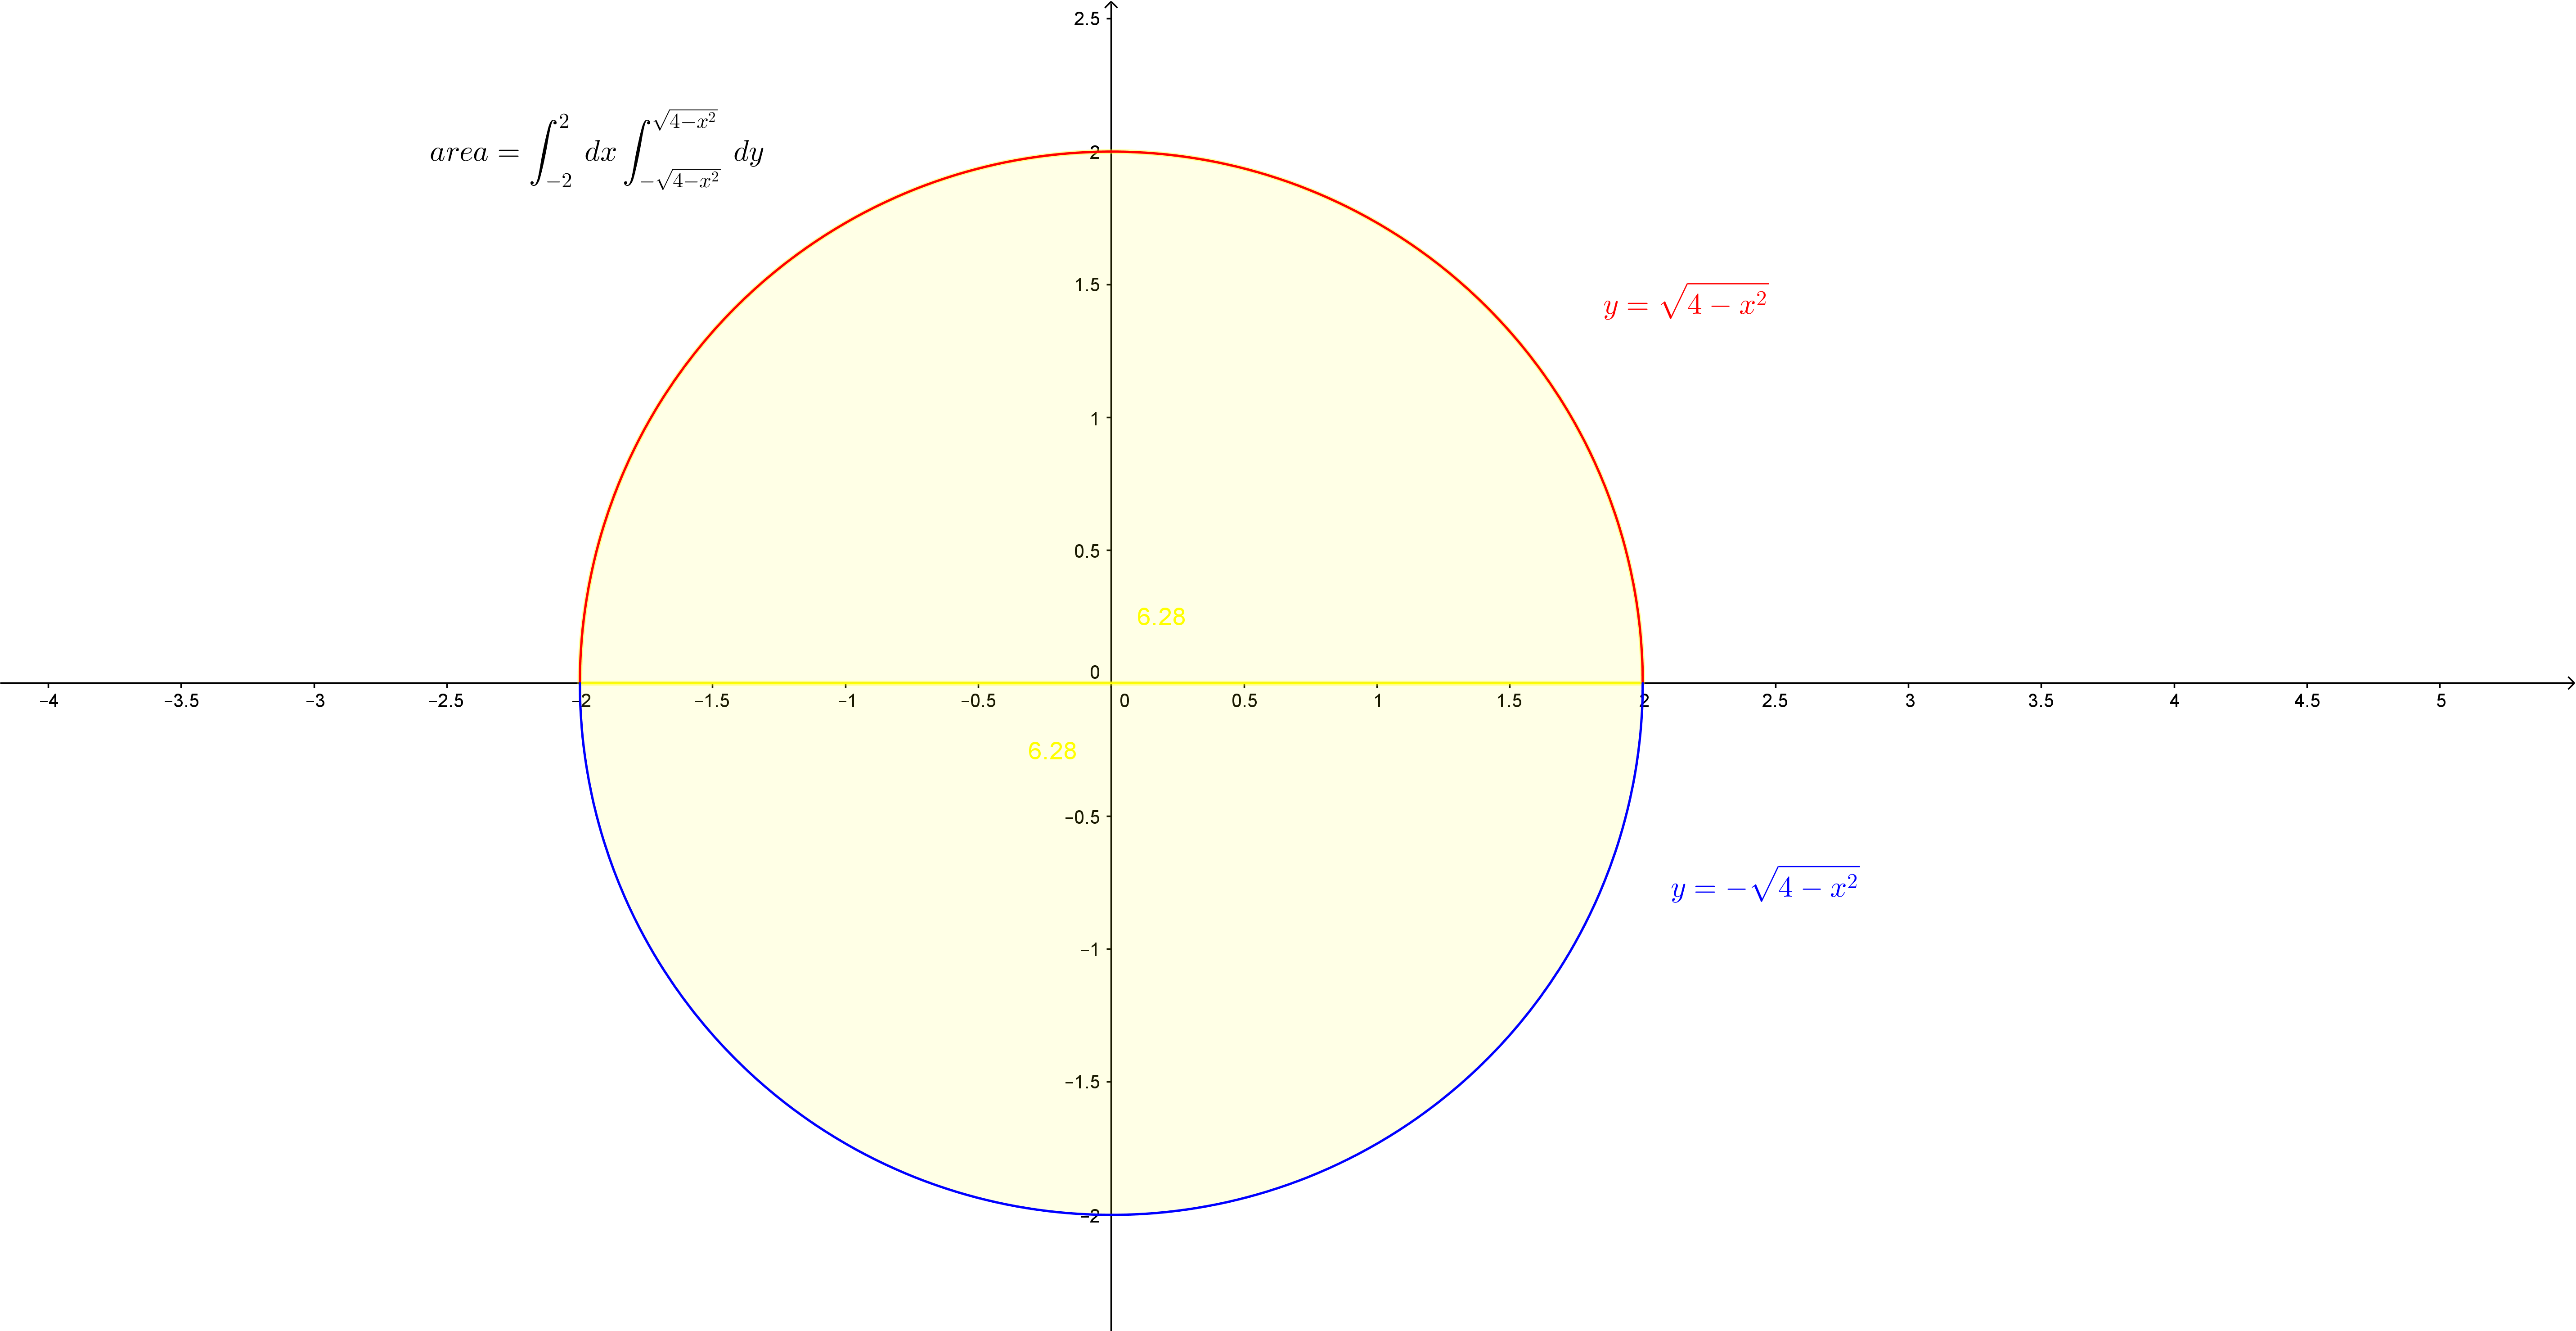
\includegraphics[width=0.5\textwidth]{v11_a01_e01.png}		
	\end{figure}
	
	\begin{equation*}
		r = 2 \Rightarrow a = \pi r^2 = 2^2 \pi = 4\pi	
	\end{equation*}
	\begin{equation*}
		x^2 + y^2 = r^2 \Rightarrow x^2 + y^2 = 2^2 \Rightarrow x^2 + y^2 = 4 \Rightarrow y = \pm\sqrt{4 - x^2}
	\end{equation*}	
	\begin{equation*}
		R = \left\{(x, y) \in \mathbb{R}^2 \,|\, -2 \leq x \leq 2,\, -\sqrt{4 - x^2} \leq y \leq \sqrt{4 - x^2} \right\}
	\end{equation*}
	\begin{gather*}
		a = \int_{-2}^2 dx \int_{-\sqrt{4 - x^2}}^{\sqrt{4 - x^2}} dy = \int_{-2}^2 dx \left(\sqrt{4 - x^2} + \sqrt{4 - x^2}\right) = 2\int_{-2}^2 \sqrt{4 - x^2}\, dx =\\ 2\int_{-2}^2 \sqrt{4 - (2\sen(\alpha))^2}\, 2\cos(\alpha)\,d\alpha = 4\int_{-2}^2 \sqrt{4 - 4\sen^2(\alpha)}\, \cos(\alpha)\,d\alpha =\\ 4\int_{-2}^2 \sqrt{4 - 4\left(1 - \cos^2(\alpha)\right)}\, \cos(\alpha)\,d\alpha = 4\int_{-2}^2 \sqrt{4 - \left(4 - 4\cos^2(\alpha)\right)}\, \cos(\alpha)\,d\alpha =\\ 4\int_{-2}^2 \sqrt{\overstrike{4 - 4} + 4\cos^2(\alpha)}\, \cos(\alpha)\,d\alpha = 4\int_{-2}^2 2\cos(\alpha)\cos(\alpha)\,d\alpha =\\ 8\int_{-2}^2 \cos^2(\alpha)\,d\alpha = 8\int_{-2}^2 \left(\dfrac{1 + \cos(2\alpha)}{2}\right)\,d\alpha = 8\int_{-2}^2 \left(\dfrac{1}{2} + \dfrac{\cos(2\alpha)}{2}\right)\,d\alpha =\\ 4\int_{-2}^2 d\alpha + 4\int_{-2}^2 \cos(2\alpha)\, d\alpha = 4\int_{-2}^2 d\alpha + 4\int_{-2}^2 \cos(u)\, \dfrac{du}{2} =\\ 4\int_{-2}^2 d\alpha + 2\int_{-2}^2 \cos(u)\, du = \left[4\alpha + 2 \sen(u)\right]_{-2}^2 = \left[4\alpha + 2 \sen(2\alpha)\right]_{-2}^2 =\\ \left[4\alpha + 4 \sen(\alpha)\cos(\alpha)\right]_{-2}^2 = \left[4\left(\alpha + \sen(\alpha)\cos(\alpha)\right)\right]_{-2}^2 =\\ \left[4\left(\arcsen\left(\dfrac{x}{2}\right) + \dfrac{x}{2}\dfrac{\sqrt{4 - x^2}}{2}\right)\right]_{-2}^2 = \left[4\left(\arcsen\left(\dfrac{x}{2}\right) + \dfrac{x\sqrt{4 - x^2}}{4}\right)\right]_{-2}^2 =\\ 4\left(\arcsen\left(\dfrac{2}{2}\right) + \dfrac{2\sqrt{4 - 2^2}}{4}\right) - 4\left(\arcsen\left(\dfrac{(-2)}{2}\right) + \dfrac{(-2)\sqrt{4 - (-2)^2}}{4}\right) =\\ 4\arcsen(1) - 4\arcsen(-1) =  4(\arcsen(1) - \arcsen(-1)) = 4\left(\dfrac{\pi}{2} + \dfrac{\pi}{2}\right) = 4\left(\dfrac{\overstrike{2}\pi}{\overstrike{2}}\right) = 4\pi
	\end{gather*}
	\begin{equation*}
		x = 2\sen(\alpha);\; dx = 2\cos(\alpha)\,d\alpha
	\end{equation*}
	\begin{equation*}
		u = 2\alpha;\; \dfrac{du}{2} = d\alpha
	\end{equation*}
	\begin{equation*}
		\sen(\alpha) = \dfrac{co}{h} = \dfrac{x}{2} \Rightarrow \alpha = \arcsen\left(\dfrac{x}{2}\right)
	\end{equation*}
	\begin{equation*}
		h^2 = co^2 + ca^2 \Rightarrow 2^2 = x^2 + ca^2 \Rightarrow ca = \sqrt{4 - x^2}
	\end{equation*}
	\begin{equation*}
		\cos(\alpha) = \dfrac{ca}{h} = \dfrac{\sqrt{4 - x^2}}{2}
	\end{equation*}
	\begin{equation*}
		R = \left\{(r, \theta) \in \mathbb{R}^2 \,|\, 0 \leq r \leq 2,\, 0 \leq \theta \leq 2\pi \right\}
	\end{equation*}
	\begin{gather*}
		a = \int_{-2}^2 dx \int_{-\sqrt{4 - x^2}}^{\sqrt{4 - x^2}} dy = \int_0^2 \int_0^{2\pi} r\, drd\theta = \int_0^2 r\, dr \int_0^{2\pi} d\theta = \left[\dfrac{r^2}{2}\right]_0^2 [\theta]_0^{2\pi} =\\ \dfrac{1}{2}\left[2^2 - 0^2\right][2\pi - 0] = \dfrac{4}{\overstrike{2}}\overstrike{2}\pi = 4\pi
	\end{gather*}
		
	\item Exercício
	
	\begin{equation*}
		\iint_R \dfrac{da}{1 + x^2 + y^2}
	\end{equation*}
	
	\begin{figure}[htb]
		\caption{Coordenadas polares - Aula 01 - Exercício II}
		\label{v11_a01_e02}
		\centering
		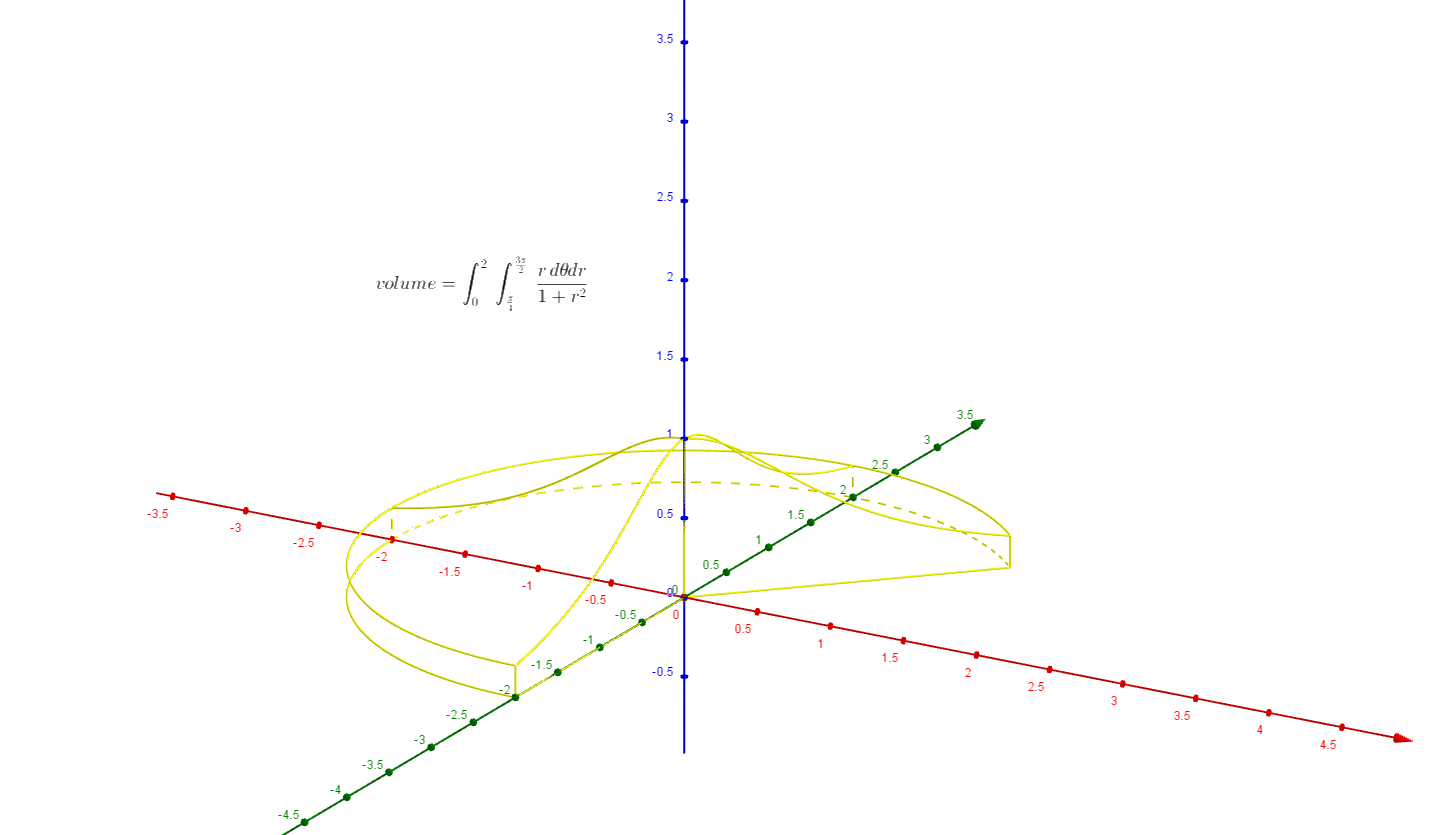
\includegraphics[width=0.5\textwidth]{v11_a01_e02.png}		
	\end{figure}
	
	\begin{equation*}
		R = \left\{(r, \theta) \in \mathbb{R}^2 \,|\, 0 \leq r \leq 2,\, \dfrac{\pi}{4} \leq \theta \leq \dfrac{3\pi}{2} \right\}
	\end{equation*}
	\begin{gather*}
		v = \iint_R \dfrac{da}{1 + x^2 + y^2} = \int_0^2 \int_{\frac{\pi}{4}}^{\frac{3\pi}{2}} \dfrac{r\, drd\theta}{1 + r^2} = \int_0^2 \dfrac{r\, dr}{1 + r^2} \int_{\frac{\pi}{4}}^{\frac{3\pi}{2}} d\theta =\\ \int_0^2 \left(1 + r^2\right)^{-1} r\, dr \left[\theta\right]_{\frac{\pi}{4}}^{\frac{3\pi}{2}} = \int_0^2 \left(1 + r^2\right)^{-1} r\, dr \left(\dfrac{3\pi}{2} - \dfrac{\pi}{4}\right) =\\ \int_0^2 \left(1 + r^2\right)^{-1} r\, dr\left(\dfrac{6\pi - \pi}{4}\right) = \dfrac{5\pi}{4}\int_0^2 \left(1 + r^2\right)^{-1} r\, dr = \dfrac{5\pi}{4}\int_0^2 u^{-1} \dfrac{du}{2} =\\ \dfrac{5\pi}{8}\int_0^2 u^{-1} du = \dfrac{5\pi}{8}\left[ln |u|\right]_0^2 = \dfrac{5\pi}{8}\left[ln |1 + r^2|\right]_0^2 = \dfrac{5\pi}{8}\left[ln |1 + 2^2| - ln |1 + 0^2|\right] =\\ \dfrac{5\pi}{8}\left[ln |5| - ln |1|\right] = \dfrac{5\pi ln |5|}{8}
	\end{gather*}
	\begin{equation*}
		u = 1 + r^2 \Rightarrow \dfrac{du}{2} = r\,dr
	\end{equation*}
	\begin{equation*}
		\e^x = 1 = \e^0 \Rightarrow x = 0
	\end{equation*}
\end{enumerate}

	%\subsection{Aula 2}
	
	%\subsection{Aula 3}

\chapter{Integrais triplas}\label{integrais_triplas}
\chapterprecis{Cálculo de integrais triplas.}\index{sinopse de capítulo}	
	%\section{Introdução - Aula 1}
	
	%\section{Cálculo de integrais triplas - Aula 2}
	
	%\section{Cálculo do volume de um sólido - Aula 3}
	
	%\section{Esboço de um sólido - Aula 4}
	
	%\section{Coordenadas esféricas}
	%\subsection{Aula 1}
	
	%\subsection{Aula 2}
	
	%\subsection{Aula 3}
	
	%\subsection{Aula 4}
	
	%\subsection[Aula 5]{Cálculo de massa com coordenadas esféricas - Aula 5}
	
	%\subsection{Aula 6}
	
	%\subsection{Aula 7}
	
	%\section{Coordenadas cilíndricas}
	%\subsection{Aula 1}
	
	%\subsection{Aula 2}
	
	%\subsection{Aula 3}
	
	%\subsection{Aula 4}
	
	%\subsection{Aula 5}
	
	%\subsection{Aula 6}
	
	%\subsection{Aula 7}
	
	%\subsection{Aula 8}

%\subsection{Aula 2}

%\subsection{Aula 3}

% ----------------------------------------------------------
% ELEMENTOS PÓS-TEXTUAIS
% ----------------------------------------------------------
\postextual

% ----------------------------------------------------------
% Referências bibliográficas
% ----------------------------------------------------------
\bibliography{referencia}

% ----------------------------------------------------------
% Anexos
% ----------------------------------------------------------

% ---
% Inicia os anexos
% ---
\begin{anexosenv}
	
	% Imprime uma página indicando o início dos anexos
	\partanexos
	
	% ---
	\chapter{Derivadas}
	% ---
	\label{anexo_derivadas}
	\subsection{Derivadas simples}
	\begin{table}[H]
		\centering
		\begin{tabular}{|lclclcl|}
			$y$ & $=$ & $c$            & $\Rightarrow$ & $y'$ & $=$ & $0$                       \\
			$y$ & $=$ & $x$            & $\Rightarrow$ & $y'$ & $=$ & $1$                       \\
			$y$ & $=$ & $x^c$          & $\Rightarrow$ & $y'$ & $=$ & $cx^{c - 1}$              \\
			$y$ & $=$ & $\e^x$         & $\Rightarrow$ & $y'$ & $=$ & $\e^x$                    \\
			$y$ & $=$ & $\ln |x|$      & $\Rightarrow$ & $y'$ & $=$ & $\dfrac{1}{x}$            \\
			$y$ & $=$ & $uv$           & $\Rightarrow$ & $y'$ & $=$ & $u'v + uv'$               \\
			$y$ & $=$ & $\dfrac{u}{v}$ & $\Rightarrow$ & $y'$ & $=$ & $\dfrac{u'v - uv'}{v^2}$  \\
			$y$ & $=$ & $u^c$          & $\Rightarrow$ & $y'$ & $=$ & $cu^{c - 1}u'$            \\
			$y$ & $=$ & $\e^u$         & $\Rightarrow$ & $y'$ & $=$ & $\e^uu'$                  \\
			$y$ & $=$ & $c^u$          & $\Rightarrow$ & $y'$ & $=$ & $c^uu'ln|c|$              \\
			$y$ & $=$ & $\ln |u|$      & $\Rightarrow$ & $y'$ & $=$ & $\dfrac{u'}{u}$           \\
			$y$ & $=$ & $\log_c|u|$    & $\Rightarrow$ & $y'$ & $=$ & $\dfrac{u'}{u}\log_c|\e|$
		\end{tabular}
		\caption{Derivadas simples}
		\label{derivadas_simples}
	\end{table}

\subsection{Derivadas trigonométricas}
	\begin{table}[H]
		\centering
		\begin{tabular}{|lclclcl|}
			$y$ & $=$ & $\sen(x)$       & $\Rightarrow$ & $y'$ & $=$ & $\cos(x)$                       \\
			$y$ & $=$ & $\cos(x)$       & $\Rightarrow$ & $y'$ & $=$ & $-\sen(x)$                      \\
			$y$ & $=$ & $\tg(x)$        & $\Rightarrow$ & $y'$ & $=$ & $\sec^2(x)$                     \\
			$y$ & $=$ & $\cotg(x)$      & $\Rightarrow$ & $y'$ & $=$ & $-\cossec^2(x)$                 \\
			$y$ & $=$ & $\sec(x)$       & $\Rightarrow$ & $y'$ & $=$ & $\sec(x)\tg(x)$                 \\
			$y$ & $=$ & $\cossec(x)$    & $\Rightarrow$ & $y'$ & $=$ & $-\cossec(x)\cotg(x)$           \\
			$y$ & $=$ & $\arcsen(x)$    & $\Rightarrow$ & $y'$ & $=$ & $\dfrac{1}{\sqrt{1 - x^2}}$     \\
			$y$ & $=$ & $\arccos(x)$    & $\Rightarrow$ & $y'$ & $=$ & $\dfrac{-1}{\sqrt{1 - x^2}}$    \\
			$y$ & $=$ & $\arctg(x)$     & $\Rightarrow$ & $y'$ & $=$ & $\dfrac{1}{1 + x^2}$            \\
			$y$ & $=$ & $\arccotg(x)$   & $\Rightarrow$ & $y'$ & $=$ & $\dfrac{-1}{1 + x^2}$           \\
			$y$ & $=$ & $\arcsec(x)$    & $\Rightarrow$ & $y'$ & $=$ & $\dfrac{1}{|x|\sqrt{x^2 - 1}}$  \\
			$y$ & $=$ & $\arccossec(x)$ & $\Rightarrow$ & $y'$ & $=$ & $\dfrac{-1}{|x|\sqrt{x^2 - 1}}$
		\end{tabular}
		\caption{Derivadas trigonométricas}
		\label{derivadas_trigometricas}
	\end{table}
	
	% ---
	\chapter{Integrais}
	% ---
	
	\label{anexo_integrais}
	\section{Integrais simples}
	\begin{table}[H]
		\caption{Integrais simples}
		\label{integrais_simples}
		\centering
		\begin{tabular}{|lclcr|}
			$\displaystyle\int dx$            & $=$ & $x + c$                       &               &  \\
			$\displaystyle\int x^p\, dx$      & $=$ & $\dfrac{x^{p + 1}}{p+ 1} + c$ & $\rightarrow$ & $p\neq -1$ \\
			$\displaystyle\int \e^x\, dx$     & $=$ & $\e^x + c$                    &               &  \\
			$\displaystyle\int \dfrac{dx}{x}$ & $=$ & $\ln|x| + c$                  &               &  \\
			$\displaystyle\int u^p\, du$      & $=$ & $\dfrac{u^{p + 1}}{p+ 1} + c$ & $\rightarrow$ & $p\neq -1$ \\
			$\displaystyle\int \e^u\, du$     & $=$ & $\e^u + c$                    &               &  \\
			$\displaystyle\int \dfrac{du}{u}$ & $=$ & $\ln|u| + c$                  &               &  \\
			$\displaystyle\int p^u\, du$      & $=$ & $\dfrac{p^u}{\ln|p|} + c$     &               &
		\end{tabular}		
	\end{table}

\section{Integrais trigonométricas}
	\begin{table}[H]
		\caption{Integrais trigonométricas}
		\label{integrais_trigonometricas}
		\centering
		\begin{tabular}{|lcl|}
			$\displaystyle\int \sen(u)du$                      & $=$ & $-\cos(u) + c$                   \\
			$\displaystyle\int \cos(u)du$                      & $=$ & $\sen(u) + c$                    \\
			$\displaystyle\int \tg(u)du$                       & $=$ & $\ln|\sec(u)| + c$               \\
			$\displaystyle\int \cotg(u)du$                     & $=$ & $\ln|\sen(u)| + c$               \\
			$\displaystyle\int \sec(u)du$                      & $=$ & $\ln|\sec(u) + \tg(u)| + c$      \\
			$\displaystyle\int \cossec(u)du$                   & $=$ & $\ln|\cossec(u) - \cotg(u)| + c$ \\
			$\displaystyle\int \sec^2(u)du$                    & $=$ & $\tg(u) + c$                     \\
			$\displaystyle\int \cossec^2(u)du$                 & $=$ & $-\cotg(u) + c$                  \\
			$\displaystyle\int \sec(u)\tg(u)du$                & $=$ & $\sec(u) + c$                    \\
			$\displaystyle\int \cossec(u)\cotg(u)du$           & $=$ & $-\cossec(u) + c$                \\
			$\displaystyle\int \dfrac{du}{\sqrt{1 - x^2}}$     & $=$ & $\arcsen(x) + c$                 \\
			$-\displaystyle\int \dfrac{du}{\sqrt{1 - x^2}}$    & $=$ & $\arccos(x) + c$                 \\
			$\displaystyle\int \dfrac{du}{1 + x^2}$            & $=$ & $\arctg(x) + c$                  \\
			$-\displaystyle\int \dfrac{du}{1 + x^2}$           & $=$ & $\arccotg(x) + c$                \\
			$\displaystyle\int \dfrac{du}{|x|\sqrt{x^2 - 1}}$  & $=$ & $\arcsec(x) + c$                 \\
			$-\displaystyle\int \dfrac{du}{|x|\sqrt{x^2 - 1}}$ & $=$ & $\arccossec(x) + c$
		\end{tabular}		
	\end{table}

\section{Relação entre coordenadas cartesinas e polares}
	\begin{figure}[H]
		\caption{Coordenadas cartesinas e polares}
		\label{coordenadas_cartesianas_polares}
		\centering
		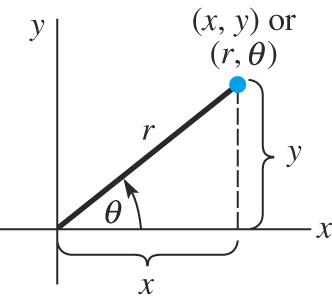
\includegraphics[width=0.5\textwidth]{coordenadas_polares.jpg}		
	\end{figure}
		
	$$r \in [0, \infty),\, \theta \in [0,\, 2\pi]$$
	
	\begin{table}[H]
		\caption{Transformação de coordenadas cartesinas em polares}
		\label{transformacao_coordenadas_cartesianas_polares}
		\centering		
		\begin{tabular}{|lclclcl|}
			$\theta$       & $=$ & $\arctg\left(\dfrac{y}{x}\right)$ & $\Rightarrow$ & $\dfrac{y}{x}$ & $=$ & $\tg(\theta)$     \\
			$\sen(\theta)$ & $=$ & $\dfrac{y}{r}$                    & $\Rightarrow$ & $y$            & $=$ & $r\,\sen(\theta)$ \\
			$\cos(\theta)$ & $=$ & $\dfrac{x}{r}$                    & $\Rightarrow$ & $x$            & $=$ & $r\,\cos(\theta)$
		\end{tabular}		
	\end{table}
	\begin{table}[H]
		\caption{Coordenadas polares a partir das suas correspondentes cartesianas}
		\label{correpondentes_coordenadas_cartesianas_polares}
		\centering		
		\begin{tabular}{|lclclcl|}
			$x^2 + y^2$    & $=$ & $r^2$          & $\Rightarrow$ & $r$      & $=$ & $\sqrt{x^2 + y^2}$                 \\
			$\sen(\theta)$ & $=$ & $\dfrac{y}{r}$ & $\Rightarrow$ & $\theta$ & $=$ & $\arcsen\left(\dfrac{y}{r}\right)$ \\
			$\cos(\theta)$ & $=$ & $\dfrac{x}{r}$ & $\Rightarrow$ & $\theta$ & $=$ & $\arccos\left(\dfrac{x}{r}\right)$
		\end{tabular}		
	\end{table}
	
	\begin{equation*}
		v = \iint_{R(x,y)} f(x,y)\, dxdy = \iint_{R(r,\theta)} f(r\,\cos(\theta),\,r\,\sen(\theta)) r\,drd\theta
	\end{equation*}
	
\section{Relação entre coordenadas cartesinas e esféricas}
	
	\begin{figure}[H]
		\caption{Coordenadas esféricas}
		\label{coordenadas_esfericas}
		\centering
		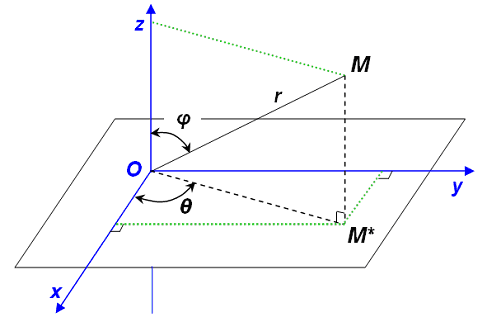
\includegraphics[width=0.5\textwidth]{coordenadas_esfericas.png}		
	\end{figure}
	
	$$r \in [0, \infty),\, \varphi \in [0,\, \pi],\, \theta \in [0,\, 2\pi]$$
	
	\begin{table}[H]
		\caption{Transformação de coordenadas cartesinas em esféricas}
		\label{transformacao_coordenadas_cartesianas_esfericas}
		\centering		
		\begin{tabular}{|lclclcl|}
			$\sen(\varphi)\cos(\theta)$ & $=$ & $\dfrac{x}{r}$ & $\Rightarrow$ & $x$ & $=$ & $r\,\sen(\varphi)\cos(\theta)$ \\
			$\sen(\varphi)\sen(\theta)$ & $=$ & $\dfrac{y}{r}$ & $\Rightarrow$ & $y$ & $=$ & $r\,\sen(\varphi)\sen(\theta)$ \\
			$\cos(\varphi)$             & $=$ & $\dfrac{z}{r}$ & $\Rightarrow$ & $z$ & $=$ & $r\,\cos(\varphi)$
		\end{tabular}		
	\end{table}	
	\begin{table}[H]
		\caption{Coordenadas esféricas a partir das suas correspondentes cartesianas}
		\label{correpondentes_coordenadas_cartesianas_esfericas}
		\centering		
		\begin{tabular}{|lclclcl|}
			$x^2 + y^2 + z^2$ & $=$ & $r^2$                         & $\Rightarrow$ & $r$       & $=$ & $\sqrt{x^2 + y^2 + z^2}$                         \\
			$\tg(\theta)$     & $=$ & $\dfrac{y}{x}$                & $\Rightarrow$ & $\theta$  & $=$ & $\arctg\left(\dfrac{y}{x}\right)$                \\
			$\tg(\varphi)$    & $=$ & $\dfrac{\sqrt{x^2 + y^2}}{z}$ & $\Rightarrow$ & $\varphi$ & $=$ & $\arctg\left(\dfrac{\sqrt{x^2 + y^2}}{z}\right)$
		\end{tabular}		
	\end{table}
	
	\begin{align*}
		v = \iiint_{R(x,y,z)} f(x,y,z)\, dxdydz =\\ \iiint_{R(r,\theta,\varphi)} f(r\,\sen(\varphi)\cos(\theta),\, r\,\sen(\varphi)\sen(\theta),\, r\,\cos(\varphi))\, r^2\sen(\varphi)\, dr d\varphi d\theta
	\end{align*}
	
	% ---
	\chapter{Funções trigonométricas}
	% ---
	
	\label{anexo_funcoes_trigonometricas}
	\section{Determinação do seno, cosseno e tangente}
	\begin{figure}[H]
		\caption{Determinação do seno, cosseno e tangente}
		\label{triangulo_retangulo}
		\centering
		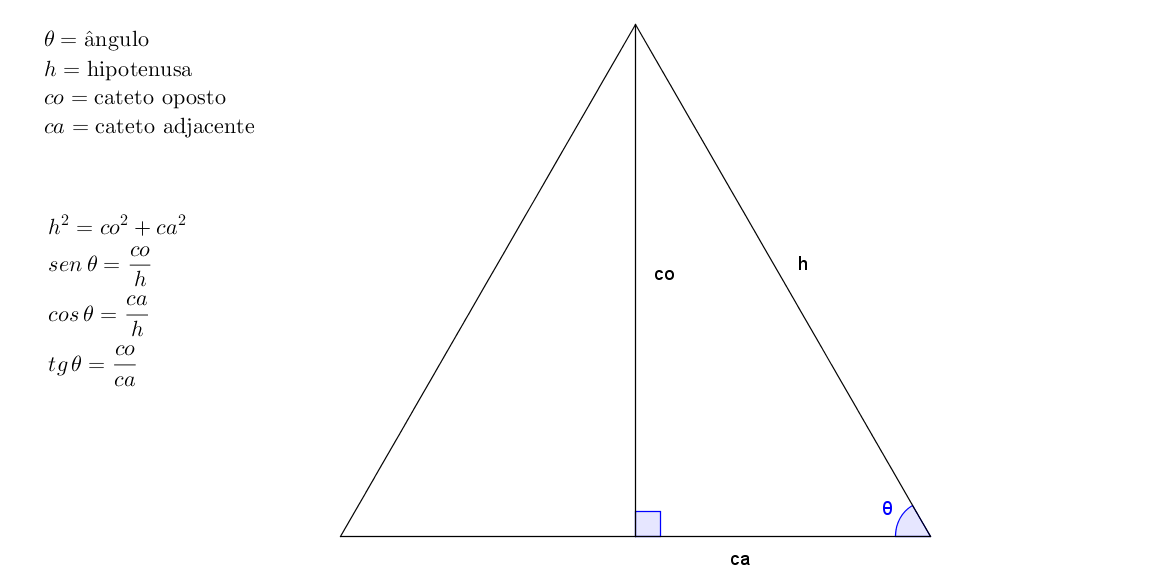
\includegraphics[width=0.5\textwidth]{triangulo_retangulo.png}		
	\end{figure}
	
\section{Círculo trigonométrico}
	\begin{figure}[H]
		\caption{Círculo trigonométrico}
		\label{circulo_trigonometrico}
		\centering
		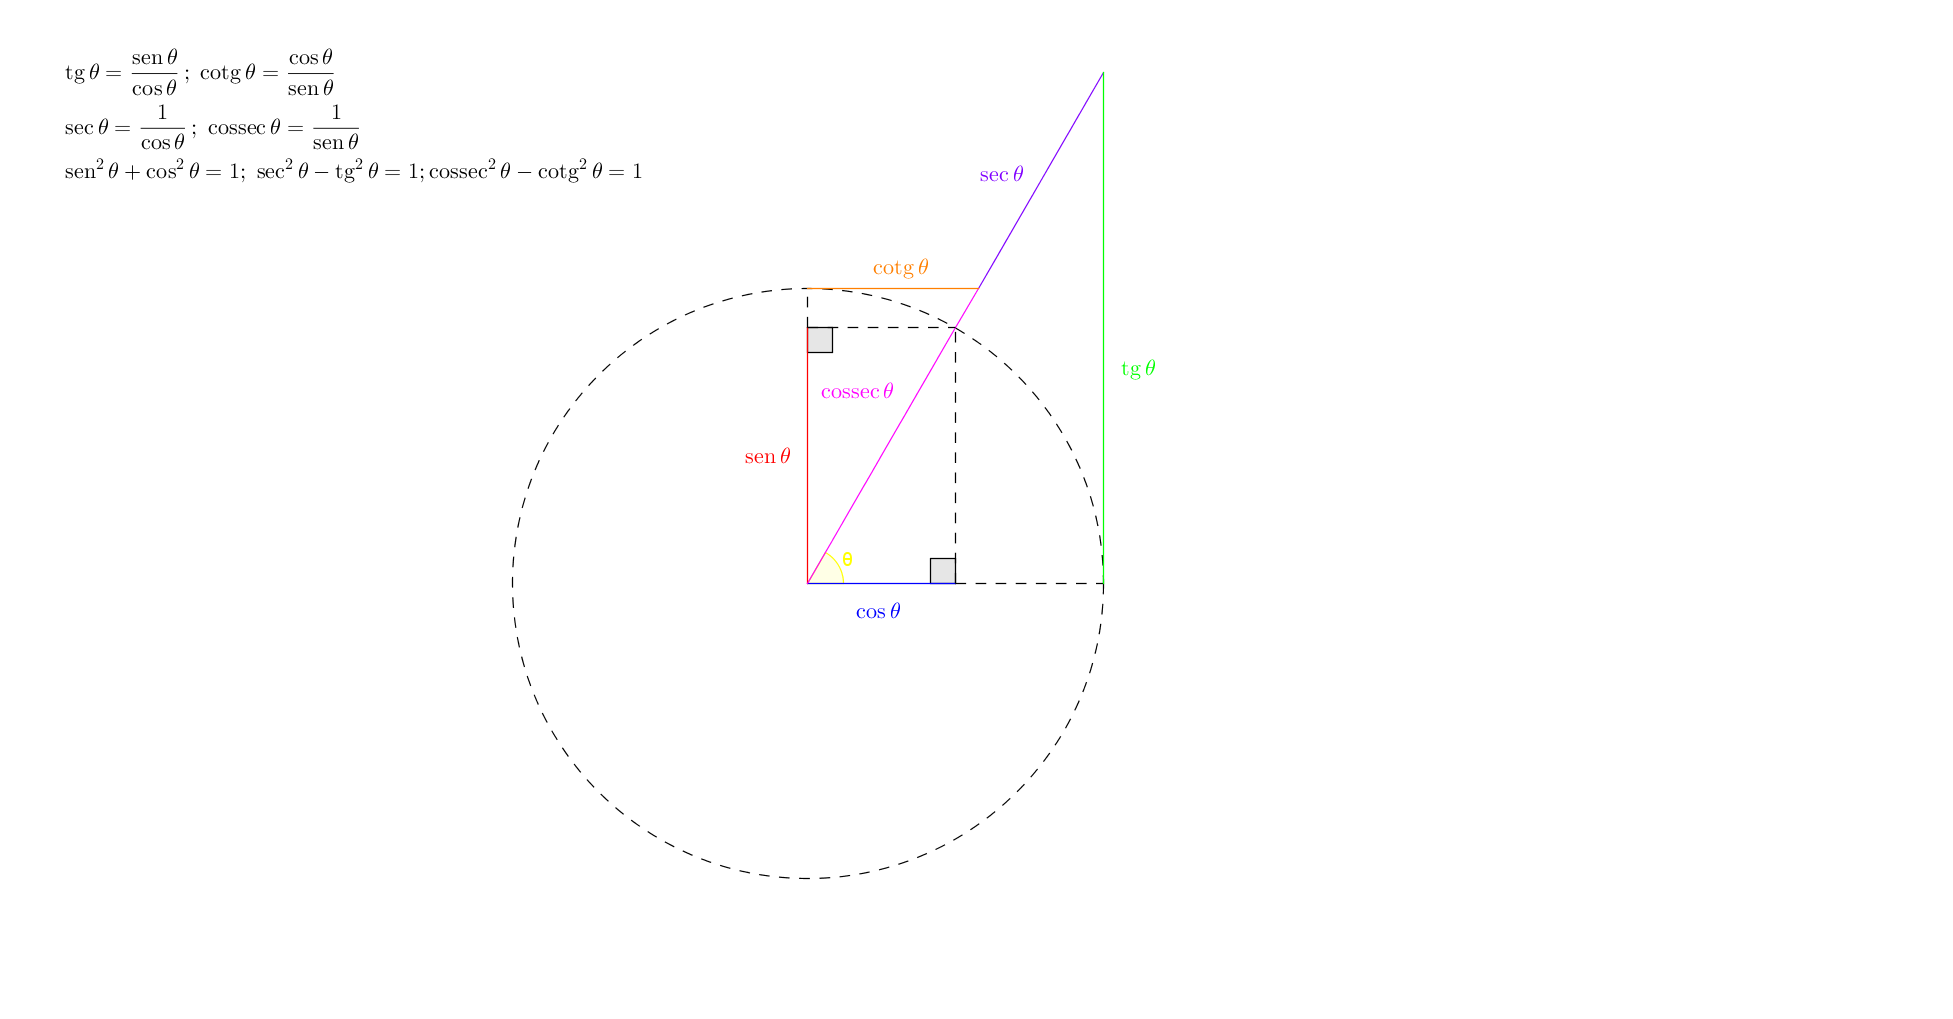
\includegraphics[width=0.5\textwidth]{circulo_trigonometrico.png}		
	\end{figure}
	
\section{Identidades trigonométricas}
	\begin{table}[H]
		\caption{Identidades trigonométricas}
		\label{identidades_trigonometricas}
		\centering
		\begin{tabular}{|lcl|}
			$\tg(x)$                    & $=$ & $\dfrac{\sen(x)}{\cos(x)}$ \\
			$\cotg(x)$                  & $=$ & $\dfrac{\cos(x)}{\sen(x)}$ \\
			$\sec(x)$                   & $=$ & $\dfrac{1}{\cos(x)}$       \\
			$\cossec(x)$                & $=$ & $\dfrac{1}{\sen(x)}$       \\
			$\sen^2(x) + \cos^2(x)$     & $=$ & $1$                        \\
			$\sec^2(x) - \tg^2(x)$      & $=$ & $1$                        \\
			$\cossec^2(x) - \cotg^2(x)$ & $=$ & $1$                        \\
			$\sen^2(x)$                 & $=$ & $\dfrac{1 - \cos(2x)}{2}$  \\
			$\cos^2(x)$                 & $=$ & $\dfrac{1 + \cos(2x)}{2}$  \\
			$\sen(2x)$                  & $=$ & $2\sen(x)\cos(x)$          \\
			$\cos(2x)$                  & $=$ & $\cos^2(x) - \sen^2(x)$
		\end{tabular}		
	\end{table}
	
\section{Relação entre trigonométricas e inversas}
	\begin{table}[H]
		\caption{Relação entre trigonométricas e inversas}
		\label{relacao_trigonometricas_inversas}
		\centering
		\begin{tabular}{|lclclcl|}
			$\sen (\theta)$    & $=$ & $x$ & $\Rightarrow$ & $\theta$ & $=$ & $\arcsen (x)$    \\
			$\cos (\theta)$    & $=$ & $x$ & $\Rightarrow$ & $\theta$ & $=$ & $\arccos (x)$    \\
			$\tg (\theta)$     & $=$ & $x$ & $\Rightarrow$ & $\theta$ & $=$ & $\arctg (x)$     \\
			$\cossec (\theta)$ & $=$ & $x$ & $\Rightarrow$ & $\theta$ & $=$ & $\arccossec (x)$ \\
			$\sec (\theta)$    & $=$ & $x$ & $\Rightarrow$ & $\theta$ & $=$ & $\arcsec (x)$    \\
			$\cotg (\theta)$   & $=$ & $x$ & $\Rightarrow$ & $\theta$ & $=$ & $\arccotg (x)$
		\end{tabular}		
	\end{table}

\section{Substituição trigonométrica}
	\begin{table}[H]
		\caption{Substituição trigonométrica}
		\label{substituicao_trigonometrica}
		\centering
		\begin{tabular}{|lclcl|}
			$\sqrt{a^2 - x^2}$ & $\Rightarrow$ & $x$ & $=$ & $a\sen (\theta)$ \\
			$\sqrt{a^2 + x^2}$ & $\Rightarrow$ & $x$ & $=$ & $a\tg (\theta)$  \\
			$\sqrt{x^2 - a^2}$ & $\Rightarrow$ & $x$ & $=$ & $a\sec (\theta)$
		\end{tabular}		
	\end{table}

\section{Ângulos notáveis}
	\begin{table}[H]
		\caption{Ângulos notáveis}
		\label{angulos_notaveis}
		\centering
		\begin{tabular}{|l|l|l|l|l|l|}
			\hline
			ângulo & $0^\circ\, (0)$ & $30^\circ\, \left(\frac{\pi}{6}\right)$ & $45^\circ\, \left(\frac{\pi}{4}\right)$ & $60^\circ\, \left(\frac{\pi}{3}\right)$ & $90^\circ\, \left(\frac{\pi}{2}\right)$ \\ \hline
			$\sen$ & $0$             & $\dfrac{1}{2}$                          & $\dfrac{\sqrt{2}}{2}$                   & $\dfrac{\sqrt{3}}{2}$                   & $1$                                     \\ \hline
			$\cos$ & $1$             & $\dfrac{\sqrt{3}}{2}$                   & $\dfrac{\sqrt{2}}{2}$                   & $\dfrac{1}{2}$                          & $0$                                     \\ \hline
			$\tg$  & $0$             & $\dfrac{\sqrt{3}}{3}$                   & $1$                                     & $\sqrt{3}$                              & $\nexists$                                \\ \hline
		\end{tabular}		
	\end{table}
	
\end{anexosenv}

%---------------------------------------------------------------------
% INDICE REMISSIVO
%---------------------------------------------------------------------

\phantompart

\printindex


\end{document}
